\RequirePackage{plautopatch}
\documentclass[dvipdfmx]{jsreport}
\usepackage{amsmath,amssymb,mathrsfs}
\usepackage{bm}
\usepackage{cite}
\usepackage{float}
\usepackage{url}
\usepackage{braket}
\usepackage{mathtools}
%%
\usepackage{amsthm}
\usepackage{slashed}
%\usepackage[numers,sort]{natbib}
\setlength{\textwidth}{\fullwidth}
\setlength{\textheight}{40\baselineskip}
\addtolength{\textheight}{\topskip}
\setlength{\voffset}{-0.2in}
\setlength{\topmargin}{-5pt}
\setlength{\headheight}{0pt}
\setlength{\headsep}{0pt}
\setlength{\textheight}{23.5cm}
\addtolength{\footskip}{3mm}
\usepackage{wrapfig}%¥図の周りに文章を回り込ませる
\usepackage[dvipdfmx]{graphicx,color}
\usepackage{pgfplots}
\pgfplotsset{compat=1.16}
\usetikzlibrary{intersections,calc,arrows.meta,decorations.pathmorphing,backgrounds,positioning,fit,petri}
\usepackage{array}
\usepackage{siunitx}
\usepackage[version=3]{mhchem}
\usepackage{physics}
\usepackage{tcolorbox}
\usepackage[dvipdfmx]{hyperref}
\usepackage{pxjahyper}
\usepackage{tikz}
\usepackage{subfigure}
\hypersetup{colorlinks=true}
%%
\numberwithin{equation}{chapter}
\numberwithin{table}{chapter}

\begin{document}
\begin{titlepage}
	\begin{center}
		
		{\large 令和4年度}
		
		\vspace{10truept}
		
		{\large 卒業論文}
		
		\vspace*{100truept}
		
%		{\huge 表面弾性波-スピン渦度結合における\\スピン軌道相互作用の寄与} 
		{\huge Rayleigh波によるスピン流生成における\\スピン軌道相互作用の寄与} 
		
		\vspace{80truept}
		
		{\LARGE 武藤永治}
		
		\vspace{5truept}
		
		{\Large 学籍番号 : 61819045}
		
		\vspace{70truept}
		
		{\Large 指導教員 : 能崎幸雄}
		
		\vspace{70truept}
		
		{\Large 慶應義塾大学}
		
		\vspace{10truept}
		
		{\Large 理工学部物理学科}
		
%		\vspace{30truept}
    
		
	\end{center}
\end{titlepage}

\setcounter{tocdepth}{3}
\tableofcontents
\clearpage

\chapter{序論}
\section{研究背景}
物質の性質のほとんどを決めているのは主に物質に含まれる電子である。
電子はマイナスの電荷を持っておりさらに角運動量であるスピンと呼ばれる内部自由度を持つ。

現代社会においてエレクトロニクスは家電製品や情報通信機器など日常生活のあらゆる場面で必要な技術となっているが、基本的にこれは物質中の電荷と電流によって駆動されている。
一方で電子のスピンを利用してきた学問領域が磁気工学(マグネティクス)であり、磁化の起源である電子スピンの性質を理解して制御することで性能の良い磁石などがつくられ、磁気工学は物性物理学の格好の応用例となった。

こうして電子の電荷とスピンがエレクトロニクスと磁気工学にそれぞれ活用された状況は1990年代にナノテクノロジーが大きく進展することによって統合されて新しい学理体系が構築された。これはスピントロニクスとよばれ、巨大磁気抵抗効果という強磁性層と非磁性層を交互に積み重ねた素子に電流を流すと電気抵抗が大きく変化する効果などで成果をあげ、またたく間に実用化された。

スピントロニクスの研究が進むにつれ電子スピンの流れであるスピン流に注目が集まるようになった。物質中でスピン流はごく短い
距離で減衰してしまうが、近年のナノテクノロジーの進展によってスピン流が減衰する距離よりも短いスケールの物性が調べられるように
なり、スピン流のもたらす現象が次々と発見されるようになった。特にスピン流による磁化反転現象によりナノサイズの強磁性体の磁化方向を磁場を印加せずにスピン流を強磁性体に流すことで制御できるようになり、磁性体を利用した新しいメモリ素子であるスピンランダムアクセスメモリ(Magnetic Random Access Memory: SpinRAM)を可能にした。

スピン流の生成方法については数多くの研究がなされている。
例えば強磁性体からの非局所スピン流注入や強磁性体の温度勾配によるスピンゼーベック効果などがある。
他にも強磁性体の磁化の歳差運動によって、接合された非磁性金属にスピン角運動量が受け渡されてスピン流が注入されるスピンポンピングや
スピン軌道相互作用(spin-orbit interaction: SOI)の大きな重金属に電流を流したときアップスピンとダウンスピンが互いに逆向きに電流と垂直方向に散乱されることでスピン流が生成されるスピンホール効果やラシュバエーデルシュタイン効果という
界面でのSOIによって空間反転対称性が破れて面内方向の電流が面直方向のスピン流に変換される効果もある。

これらの手法はすべて強磁性体、SOIの強い重金属やレアメタルを必要とし、これらを用いずにスピン流を生成することはスピントロニクスにおいて重要な課題である。

\section{先行研究}
近年、ミクロなスピン角運動量とマクロな力学的回転運動との結合であるスピン回転結合(spin-rotation coupling: SRC)によって、スピン軌道相互作用の弱い非磁性金属を用いた新たなスピン流生成理論がMatuoらによって提唱された。Matuoらは表面弾性波(surface acoustic wave: SAW)や流体運動の作る渦度と電子スピンとの相互作用であるスピン渦度結合(spin-vorticity coupling: SVC)を利用して、渦度勾配中でスピン流が生成されると説明した。

このスピン流生成方法は、Kobayasiらが\ce{Cu}/\ce{NiFe}二層膜にRayleigh型表面弾性波(R-SAW)を注入し、実証実験がなされた。
さらにKurimuneらは\ce{Cu}と\ce{Pt},\ce{Ti}におけるSAWによるSVC由来のスピン流を比較し、この方法によるスピン流生成においてSOIの影響は大きくはないと結論づけた。
\section{研究目的}
先行研究によってSAWによるSVCを介したスピン流生成が実験で検証されて報告されているが、このスピン流生成法におけるSOIの寄与については以前として明らかになっていないところも多い。そこで本研究ではスピンホール角が正の材料と負の材料を用いて生成されるスピン流の量を評価することにより、SOIの寄与について調べた。
\chapter{原理}
\section{Rayleigh波}
\subsection{弾性体のひずみテンソル}
弾性体は引っ張るたりねじったりすると変形する。
変形する前の物質の場所(固体なら格子)の座標を$\bm{r},\bm{r}'$で指定し
その本来の場所$\bm{r},\bm{r}'$ からどれだけ歪んでいるかのベクトルを
$ \bm{u},\bm{u}'$で表す。このとき弾性体が歪むことによって相対位置ベクトルは次のように変化する。
\begin{equation}
\label{eq:1}
\bm{r}'-\bm{r} \to (\bm{r}'+\bm{u}')-(\bm{r}+\bm{u})=(\bm{r}'-\bm{r})+\delta \bm{u}
.\end{equation}
$\delta \bm{u}$は場所$\bm{r},\delta \bm{r}$の関数であり、$\delta r$ の一次までで展開して行列表示すると
\begin{equation}
\label{eq:2}
\begin{pmatrix} \delta u_1\\\delta u_2\\\delta u_3 \end{pmatrix} =
\begin{pmatrix} 
\frac{\partial u_1}{\partial x_1 }&\frac{\partial u_1}{\partial x_2 }&\frac{\partial u_1}{\partial x_3} \\ \frac{\partial u_2}{\partial x_1}&\frac{\partial u_2}{\partial x_2}&\frac{\partial u_2}{\partial x_3 }\\ \frac{\partial u_3}{\partial x_1} & \frac{\partial u_3}{\partial x_2} &\frac{\partial u_3}{\partial x_3} \end{pmatrix} 
\begin{pmatrix} \delta x_1\\\delta x_2 \\ \delta x_3 \end{pmatrix} 
.\end{equation}
この行列を相対変位テンソルといい、$D(\bm{r})$ で表すと\eqref{eq:2}は次のように書かれる。
\begin{equation}
\label{eq:3}
	\delta \bm{u} = D(\bm{r}) \delta \bm{r}
.\end{equation}
$D(\bm{r})\neq 0$でないときに変位が場所により変化しており弾性体は歪んでいるという。

ここで$D$ を対称成分と反対称成分に分離する。
$\varepsilon=(D+D^{T}) /2$ および$\varphi= (D-D^{T}) /2$ を用いて
以下のように分離できる。
\begin{equation}
\label{eq:4}
	D=\varepsilon+\varphi
.\end{equation}
$\varepsilon$ はひずみテンソルと呼ばれる対称行列であり、
直交行列を使って対角化することができる。このように対角化したときの新しい座標軸は主軸と呼ばれこのときの$\varepsilon$ の対角成分
$\varepsilon_{11},\varepsilon_{22},\varepsilon_{33}$ はひずみの主値と呼ばれる。
対角和$\mathrm{Tr}\,\varepsilon$ は体積膨張率と一致し変形前の体積を$V$,変形後の体積を$V'$ とすると
\begin{equation}
\label{eq:5}
	\frac{V'-V}{V}\simeq \frac{\partial u_1}{\partial x_1} +\frac{\partial u_2}{\partial x_2} +\frac{\partial u_3}{\partial x_3} =\mathrm{div} \bm{u}=\mathrm{Tr}\,\varepsilon
.\end{equation}
一方で反対称テンソル$\varphi$ は
\begin{equation}
\label{eq:6}
\bm{\Omega'}=\frac{1}{2}\nabla \times \bm{u}
\end{equation}
を用いて次のように書ける。
\begin{equation}
\label{eq:7}
\varphi=\begin{pmatrix} 0&-\Omega'_3&\Omega'_2\\\Omega'_3&0&-\Omega'_1\\-\Omega'_2&\Omega'_1&0\\ \end{pmatrix} 
.\end{equation}
このとき
\begin{equation}
\label{eq:8}
	\varphi \delta \bm{r}=\begin{pmatrix} \Omega'_2 \delta x_3-\Omega'_3 \delta x_2\\ \Omega'_3 \delta x_1-\Omega'_1 \delta x_3\\\Omega'_1 \delta x_2- \Omega'_2 \delta x_1 \end{pmatrix} =  \bm{\Omega'}\times  \delta \bm{r}
\end{equation}
となり、これはベクトル$\bm{\Omega'}$ まわりの回転を表す。
\subsection{ひずみと応力}
物体が歪んだときに物体の内部に働く力は応力と呼ばれる。これは以下で定義される応力テンソル$\sigma_{ij}$で表される。
\begin{equation}
\label{eq:9}
	\sigma_{ij}dS_j \,:\quad \text{j軸に垂直な微小面$dS_j$ に正の側からはたらく$i$方向の力}
.\end{equation}
このとき微小体積要素$dV$に周囲から働く合力の$i$ 成分は次のように表される。
\begin{equation}
\label{eq:10}
	F_i dV = \sum_{j}^{} \frac{\partial \sigma_{ij}}{\partial x_j} dV
.\end{equation}

一般に弾性体に対してひずみと応力の関係は複雑であるが、
ひずみテンソルが一様であるときには次の定義がある。

\begin{equation}
\label{eq:11}
	\sigma_{ij}=\lambda (\mathrm{div}\bm{u})\delta_{ij}+2\mu \varepsilon_{ij}
.\end{equation}
ここで$\sigma_{ij}=\sigma_{ji}$ は応力テンソルであり、$\varepsilon_{ij}=\varepsilon_{ji}$ はひずみの対称テンソル、
$\lambda,\mu$ はそれぞれラメ係数と呼ばれる量である。
物体の弾性体としての性質はこのラメ係数を用いて表される。

例えば直方体の棒を$x$ 軸方向から単位面積あたりの力$f$ で引っ張る場合を考える。
このとき
\begin{equation}
\label{eq:12}
	\text{$x$ 方向}:\quad f=\lambda(\varepsilon_{11}+\varepsilon_{22}+\varepsilon_{33})+2\mu \varepsilon_{11}
.\end{equation}
\begin{equation}
\label{eq:13}
	\text{$y$ 方向}:\quad 0=\lambda(\varepsilon_{11}+\varepsilon_{22}+\varepsilon_{33})+2\mu \varepsilon_{22}
.\end{equation}
\begin{equation}
\label{eq:14}
	\text{$z$ 方向}:\quad 0=\lambda(\varepsilon_{11}+\varepsilon_{22}+\varepsilon_{33})+2\mu \varepsilon_{33}
.\end{equation}
なお、それ以外の成分については$\varepsilon_{ij}(i\neq j)=0$ である。
\eqref{eq:12}\eqref{eq:13}\eqref{eq:14}を足すと
\begin{equation}
\label{eq:15}
	\varepsilon_{11}+\varepsilon_{22}+\varepsilon_{33}=\frac{f}{3\lambda+2\mu}
.\end{equation}
\begin{equation}
\label{eq:16}
	\varepsilon_{11}=\frac{\lambda+\mu}{\mu(3\lambda+2\mu)}f,\quad \varepsilon_{22}=\varepsilon_{33}=-\frac{\lambda}{2\mu(3\lambda+2\mu)}f
.\end{equation}
これは$x$ 方向には引っ張った分だけ伸び、$y,z$ 方向には逆に縮むということを示している。
ここでヤング率$E$ 及びポアソン比$\nu$ が以下のように定義される。
\begin{equation}
\label{eq:17}
	E:=\frac{f}{\varepsilon_{11}},\quad \nu:=-\frac{\varepsilon_{22}}{\varepsilon_{11}}\left( =-\frac{\varepsilon_{33}}{\varepsilon_{11}} \right) 
.\end{equation}
ヤング率$E$ は引っ張るときの伸び率を表し、ポアソン比$\nu$は縦伸びに対する横縮みの比率を表す。\eqref{eq:16}を代入するとこれらはラメ係数を用いて以下のように表される。
\begin{equation}
\label{eq:18}
	E=\frac{\mu(3\lambda+2\mu)}{\lambda+\mu},\quad \nu=\frac{\lambda}{2(\lambda+\mu)}
.\end{equation}
\subsection{弾性体を伝わる波}
弾性体の位置$\bm{r}$にある微小な体積要素$dV$ の微小変位$\bm{u}(\bm{r})$ の時間発展を考える。
$\bm{r}$における質量密度を$\rho(\bm{r})$ とするとNewtonの運動方程式$m \ddot{\bm{r}}=\bm{F}$は\eqref{eq:10}
を考慮して次のように書き表される。
\begin{equation}
\label{eq:19}
	\rho(\bm{r})\frac{\partial ^2 u_i}{\partial t^2} =\sum_{k}^{} \frac{\partial \sigma_{ik}}{\partial x_k} 
.\end{equation}
ここで\eqref{eq:11}を\eqref{eq:19}に代入する。そうすると
\begin{equation}
\label{eq:20}
	\sum_{k}^{} \frac{\partial \sigma_{ik}}{\partial x_k} =\lambda \frac{\partial }{\partial x_i} (\nabla \cdot \bm{u})+2\mu \sum_{k}^{} \frac{\partial \varepsilon_{ik}}{\partial x_k} 
.\end{equation}
この最終項はさらに以下のように計算される。
\begin{align*}
	\label{eq:21}
	\sum_{k}^{} \frac{\partial \varepsilon_{ik}}{\partial x_k} &= \sum_{k}^{} \frac{\partial }{\partial x_k} \frac{1}{2}\left( \frac{\partial u_i}{\partial x_k} +\frac{\partial u_k}{\partial x_i}  \right)  \\
	&= \frac{1}{2}\left( \sum_{k}^{} \frac{\partial ^2}{\partial x_k^2}  \right)u_i+\frac{1}{2}\frac{\partial }{\partial x_i} \sum_{k}^{} \frac{\partial u_k}{\partial x_k}   \\
	&= \frac{1}{2}\nabla ^2u_i+\frac{1}{2}\frac{\partial }{\partial x_i} (\nabla \cdot \bm{u}) 
	\stepcounter{equation}\tag{\theequation} 
.\end{align*}
\eqref{eq:21}を\eqref{eq:20}に代入すると
\begin{equation}
\label{eq:22}
	\sum_{k}^{} \frac{\partial \sigma_{ik}}{\partial x_k} =(\lambda+\mu)\frac{\partial }{\partial x_i} (\nabla \cdot \bm{u})+\mu \nabla ^2u_i
.\end{equation}
\eqref{eq:22}を\eqref{eq:19}に代入することで結局以下の式が得られる。
\begin{equation}
\label{eq:23}
	\rho(\bm{r})\frac{\partial ^2\bm{u}}{\partial t^2} =(\lambda+\mu)\nabla (\nabla \cdot \bm{u})+\mu\nabla ^2\bm{u}
.\end{equation}
これはナビエの方程式と呼ばれる。

ここで無限等方媒質内の弾性平面波を考える。伝搬方向を$x$ 軸方向とすると
$\bm{u}=(u_x,u_y,u_z)$ は$x$ 及び時間$t$ の関数であり、
\begin{equation}
\label{eq:24}
	u_j(x,t)\qquad j=x:\text{縦波},\quad j=y,z:\text{横波}
.\end{equation}
\eqref{eq:24}を\eqref{eq:23}に代入して整理すると
\begin{equation}
\label{eq:25}
	\frac{\partial ^2u_x}{\partial t^2} -c_l^2 \frac{\partial ^2u_x}{\partial x^2} =0.\end{equation}
\begin{equation}
\label{eq:26}
	\frac{\partial ^2u_y}{\partial t^2} -c_t^2 \frac{\partial ^2u_y}{\partial x^2} =0
.\end{equation}
\begin{equation}
\label{eq:27}
	\frac{\partial ^2u_z}{\partial t^2} -c_t^2 \frac{\partial ^2u_z}{\partial x^2} =0.\end{equation}

ここで
\begin{equation}
\label{eq:28}
	c_l=\sqrt{\frac{\lambda+2\mu}{\rho}} ,\quad c_t=\sqrt{\frac{\mu}{\rho}} 
\end{equation}
であり、$c_l>c_t$ であるので縦波の速度の方が速い。

横波においては$\mathrm{div}\,\bm{u}=0$であり、物質の体積変化には関係しない。これに対して縦波では$\mathrm{div}\,\bm{u}\neq 0$
であり物質内の圧縮や膨張に関係する。
この互いに異なる速度で独立に伝搬する2つの波への分割はより一般の(必ずしも平面波ではない)無限空間内の弾性波の場合にも成り立つ。
\eqref{eq:23}を速度$c_l,c_t$をもって書き直してみると

\begin{equation}
\label{eq:29}
	\ddot{\bm{u}}=c_t^2 \nabla ^2\bm{u}+(c_l^2-c_t^2)\mathrm{grad}\,\mathrm{div}\,\bm{u}
.\end{equation}
ここでベクトル$\bm{u}$ を以下のように2つの部分に分解する。
\begin{equation}
\label{eq:30}
	\bm{u}=\bm{u}_l+\bm{u}_t
.\end{equation}
ただしそれぞれ次のような条件を満足する。
\begin{equation}
\label{eq:31}
\mathrm{div}\,\bm{u}_t=0
.\end{equation}
\begin{equation}
\label{eq:32}
\mathrm{rot}\,\bm{u}_l=0
.\end{equation}
このような分解した表示はベクトル解析から常に可能である。
\eqref{eq:29}に$\bm{u}=\bm{u}_t+\bm{u}_l$ を代入すると
\begin{equation}
\label{eq:33}
	\ddot{\bm{u}}_l+\ddot{\bm{u}}_t=c_{l}^2 \nabla ^2(\bm{u}_l+\bm{u}_t)+(c_l^2-c_t^2)\mathrm{grad}\,\mathrm{div}\,\bm{u}_l
.\end{equation}
両辺の発散をとれば、$\mathrm{div}\,\bm{u}_t=0$より
\begin{equation}
\label{eq:34}
	\mathrm{div}\ddot{\bm{u}}_l=c_t^2\nabla ^2\mathrm{div}\,\bm{u}_l+(c_l^2-c_t^2)\nabla ^2 \mathrm{div}\,\bm{u}_l
.\end{equation}
整理して
\begin{equation}
\label{eq:35}
	\mathrm{div}\,(\ddot{\bm{u}}_l-c_l^2\nabla ^2\bm{u}_l)=0
.\end{equation}
一方で、この表式の括弧内の$\mathrm{rot}$ をとれば\eqref{eq:32}によって$0$ となる。あるベクトルの$\mathrm{rot}$ および$\mathrm{div}$ が全空間で$0$ となるときはこのベクトルは定数を除いて恒等的に$0$ となる。よって
\begin{equation}
\label{eq:36}
	\frac{\partial ^2\bm{u}_l}{\partial t^2} -c_l^2\nabla ^2\bm{u}_l=0
.\end{equation}
同様に\eqref{eq:33}の$\mathrm{rot}$ とると、$\mathrm{rot}\,\bm{u}_l=0$ および$\mathrm{rot}\,\mathrm{grad}=0$ であるので
\begin{equation}
\label{eq:37}
	\mathrm{rot}(\ddot{\bm{u}}_t-c_t^2\nabla ^2\bm{u}_t)=0
\end{equation}
が得られる。また上の括弧内の式の$\mathrm{div}$ もまた$0$ であるから\eqref{eq:36}と同じような方程式が得られ、
\begin{equation}
\label{eq:38}
	\frac{\partial ^2\bm{u}_t}{\partial t^2} -c_t^2\nabla ^2\bm{u}_t=0
.\end{equation}

方程式\eqref{eq:36}および\eqref{eq:38}は三次元の波動方程式である。これらはそれぞれ速度$c_l$ および$c_t$ をもつ弾性波の伝播を表している。波$\bm{u}_t$ は体積変化に関係しないが($\mathrm{div}\,\bm{u}_t=0$)、波$\bm{u}_l$ は体積の圧縮や膨張を伴う。
\subsection{Rayleigh波}
ここからは物体表面付近で伝播し、深部に達しない波であるSAWについて考える。
SAWの中でも変位ベクトル$\bm{u}$ が表面に対して垂直で伝搬方向を通って引かれる平面内に横たわる波をRayleigh型表面弾性波という。

\eqref{eq:36}および\eqref{eq:38}の形の波動方程式をまとめて
\begin{equation}
\label{eq:39}
	\frac{\partial ^2u}{\partial t^2} -c^2 \nabla ^2u=0
.\end{equation}
と書いておく。ここに$u$ はベクトル$\bm{u}_l,\bm{u}_t$ のある成分であり、$c$ は対応する速度$c_l$ または$c_t$である。

弾性媒質の表面は無限平面と仮定する。この平面を$xz$ 平面としてとり、媒質は$y<0$ に渡って広がっているとする。

ここで$x$ 軸に沿って伝わっていく平面単色の表面波を考える。
すなわち$u$ として
\begin{equation}
\label{eq:40}
	u=e^{i(kx-\omega t)}f(y)
\end{equation}
という形を仮定する。そこでこれを\eqref{eq:39}に代入すれば関数$f(y)$ に対して次の方程式が得られる。
\begin{equation}
\label{eq:41}
	\frac{d^2f}{dy^2}=\left( k^2-\frac{\omega^2}{c^2} \right) f
.\end{equation}
$k^2 - \omega^2 /c^2<0$ であるならば関数$f$ として周期関数を与えてしまうことになり、
物質の内部で決して減衰することのない平面波が得られてしまう。
故に$k^2 -\omega^2 /c^2>0$ であると仮定する。このとき解$f$ は次のような形を取る。
\begin{equation}
\label{eq:42}
	f(y)=\mathrm{const}\, \exp \left( \pm y\sqrt{k^2-\frac{\omega^2}{c^2}}  \right) 
.\end{equation}
負符号の解は$y\to -\infty$ にしたがってとどめなく増大してしまう解に対応し不適であるので結局解としては次のような形になる。
\begin{equation}
\label{eq:43}
	u=\mathrm{const}\,e^{i(kx-\omega t)}e^{\kappa y}
.\end{equation}
ここで
\begin{equation}
\label{eq:44}
	\kappa = \sqrt{k^2-\frac{\omega^2}{c^2}} 
.\end{equation}
は減衰定数である。
これは物体内部に向かって指数関数的に減衰する波を表しており、表面付近を伝播する波となっている。

実際の変位ベクトル$\bm{u}$ はベクトル$\bm{u}_t$ と$\bm{u}_l$ との和になっており、それぞれの成分は
\eqref{eq:39}で$\bm{u}_l$ に対しては速度$c=c_l$ 、$\bm{u}_t$ に対しては$c=c_t$ とおいた方程式を満足する。無限媒質内の体積波の場合にはこれら2つの部分は独立に伝播していくが、表面波の場合には境界条件が存在するために独立ではなくなる。

実際の変位ベクトル$\bm{u}$を与える$\bm{u}_l$ と$\bm{u}_t$ の線型結合の係数を決定づけるためには物体表面の境界条件を考える必要があり、これより波数ベクトル
$\bm{k}$ と周波数$\omega$ との分散関係が決定され、したがって波の伝搬速度が決定される。
自由境界上では$\sigma_{ik}n_k=0$という条件が成立しなければならない。境界の法線ベクトル$\bm{n}$ は
$y$ 軸に平行であるから
\begin{equation}
\label{eq:45}
	\sigma_{xy}=\sigma_{yy}=\sigma_{zy}=0
.\end{equation}
\eqref{eq:11}より従って
\begin{equation}
\label{eq:46}
	\frac{\partial u_y}{\partial x} +\frac{\partial u_x}{\partial y} =0
.\end{equation}
\begin{equation}
\label{eq:47}
	\frac{\partial u_z}{\partial y} +\frac{\partial u_y}{\partial z} =0
.\end{equation}
\begin{equation}
\label{eq:48}
	\nu (\frac{\partial u_x}{\partial x} +\frac{\partial u_z}{\partial z} )+(1-\nu)\frac{\partial u_y}{\partial y}=0 
.\end{equation}
$u_{ij}$のすべての値は$z$ に依存しないので\eqref{eq:47}より
\begin{equation}
\label{eq:49}
	\frac{\partial u_z}{\partial y} =0
.\end{equation}
\eqref{eq:43}を用いて次のような結論を得る。
\begin{equation}
\label{eq:50}
	u_{z}=0
\end{equation}
このように表面波における変形ベクトル$\bm{u}$ は表面に対して垂直で伝播方向を通って引かれる平面内に横たわる。

横波部分$\bm{u}_t$ は条件\eqref{eq:31}すなわち
\begin{equation}
\label{eq:51}
	\frac{\partial u_{tx}}{\partial x} +\frac{\partial u_{ty}}{\partial y} =0
\end{equation}
を満足せねばならない。$u_{tx},u_{ty}$の$x,y$ 依存性は因子$\exp (ikx+\kappa_ty)$ によって決定される。
ここで$\kappa_t$ は$c=c_t$ とした\eqref{eq:44}、すなわち
\begin{equation}
\label{eq:52}
	\kappa_t=\sqrt{k^2-\frac{\omega^2}{c_t^2}} 
\end{equation}
によって与えられる。故に\eqref{eq:51}は次の等式を導く
\begin{equation}
\label{eq:53}
	iku_{tx}+\kappa_tu_{ty}=0
.\end{equation}
もしくは変形して
\begin{equation}
\label{eq:54}
	\frac{u_{tx}}{u_{ty}}=-\frac{\kappa_t}{ik}
.\end{equation}
よって$a$ をある定数として
\begin{equation}
\label{eq:55}
	u_{tx}=\kappa_ta\exp (ikx+\kappa_t y-i\omega t),\quad u_{ty}=-ika\exp (ikx + \kappa_t y -i\omega t)
.\end{equation}
縦波部分$\bm{u}_{l}$は条件\eqref{eq:32}すなわち
\begin{equation}
\label{eq:56}
\frac{\partial u_{lx}}{\partial y} -\frac{\partial u_{ly}}{\partial x} =0
.\end{equation}
を満足する。したがって
\begin{equation}
\label{eq:57}
	iku_{ly}-\kappa_lu_{lx}=0,\quad \qty(\kappa_l=\sqrt{k^2-\frac{\omega^2}{c_l^2}} )
.\end{equation}
よって$b$ を定数として以下の表式を得る。
\begin{equation}
\label{eq:58}
	u_{lx}=kb\exp (ikx+\kappa_ly-i\omega t),\quad u_{ly}=-i\kappa_lb\exp (ikx +\kappa_l y -i\omega t)
.\end{equation}

続いて\eqref{eq:46},\eqref{eq:48}を用いる。これらを速度$c_l$と$c_t$ を導入して書き換える。
\eqref{eq:28}と\eqref{eq:18}から
\begin{equation}
\label{eq:59}
	\nu=\frac{c_l^2-2c_t^2}{2(c_l^2-c_t^2)}
\end{equation}
であるので
\begin{equation}
\label{eq:60}
	\frac{\partial u_x}{\partial y} +\frac{\partial u_y}{\partial x} =0
.\end{equation}
\begin{equation}
\label{eq:61}
	c_{l}^2\frac{\partial u_y}{\partial y} +(c_l^2-2c_t^2)\frac{\partial u_x}{\partial x} =0
.\end{equation}
ここで
\begin{equation}
\label{eq:62}
	u_x=u_{lx}+u_{tx},\quad u_{y}=u_{ly}+u_{ty}
\end{equation}
と置くことができるから\eqref{eq:60}より境界$y=0$ での条件であることに注意して
\begin{equation}
\label{eq:63}
	a(k^2+\kappa^2_t)+2bk\kappa_l=0
.\end{equation}
同様に\eqref{eq:61}
から以下の式を得る。
\begin{equation}
\label{eq:64}
	2ac_t^2\kappa_tk+b\left[ c_l^2(\kappa_l^2-k^2)+2c_t^2k^2 \right] =0
.\end{equation}
この式を$c_t^2$ で割ってさらに
\begin{equation}
\label{eq:65}
	\kappa_l^2-k^2=-\frac{\omega^2}{c_l^2}=-(k^2-\kappa_t^2) \frac{c_t^2}{c_l^2}
\end{equation}
を代入すると次のような形に書くことができる。
\begin{equation}
\label{eq:66}
	2a\kappa_tk+b(k^2+\kappa_t^2)=0
.\end{equation}
$a,b$ についての同時方程式系\eqref{eq:63},\eqref{eq:66}が非自明な解を持つための条件は
\begin{equation}
\label{eq:67}
	(k^2+\kappa_t^2)^2=4k^2\kappa_t\kappa_l
.\end{equation}
両辺の平方をとって$\kappa_t^2,\kappa_l^2$ の値の置き換えを行えば
\begin{equation}
\label{eq:68}
\left( 2k^2-\frac{\omega^2}{c_t^2} \right) ^{4}=16k^{4}\left( k^2-\frac{\omega^2}{c_t^2} \right) \left( k^2-\frac{\omega^2}{c_l^2} \right) 
.\end{equation}
この方程式から$\omega$ と$k$ の関係が定まる。ここで$\xi$という無次元量を導入して次のように置くと便利である。
\begin{equation}
\label{eq:69}
	\omega=c_t k\xi
.\end{equation}
そうすると、この方程式系の両辺の$k^{8}$ の項はキャンセルされ、展開すると結局次のような$\xi$ の代数方程式が得られる。
\begin{equation}
\label{eq:70}
	\xi^{6}-8\xi^{4}+8\xi^2\left( 3-2 \frac{c_t^2}{c_l^2} \right) -16\left( 1- \frac{c_t^2}{c_l^2} \right) =0
.\end{equation}
ここからわかる重要なことは$\xi$ が$c_t /c_l$という比の値だけに依存し、これはある与えられた物質に対して一定であり、言い換えればポアソン係数だけに依存するという特徴を持つことである。
すなわち
\begin{equation}
\label{eq:71}
	\frac{c_t}{c_l}=\sqrt{\frac{1-2\nu}{2(1-\nu)}} 
.\end{equation}
$\xi$ はもちろん正の実数値をとり、$\kappa_t,\kappa_l$ が実数であるために$\xi<1$ である。
方程式\eqref{eq:70}はそのような条件を満たす根を唯一つ持ち、したがって与えられた$c_t /c_l$ に対して$\xi$ の値はただ一つしか得られる。

以上より表面波でも体積波でも周波数は波数ベクトルの大きさ$k$ に比例し、その比例係数$U$ は波の伝搬速度であり
\begin{equation}
\label{eq:72}
	U=c_t\xi
.\end{equation}
これは表面弾性波(SAW)の伝播速度であり、体積波の横波および縦波速度$c_l,c_t$ によって与えられる。
横波部分と縦波部分の振幅比は\eqref{eq:66}に$\kappa_t^2=k^2-\omega^2 /c_t^2=k^2(1-\xi^2)$を代入すると($k>0$ であることに注意して)以下のように与えられる。
\begin{equation}
\label{eq:73}
	\frac{a}{b}=-\frac{2-\xi^2}{2\sqrt{1-\xi^2} }
.\end{equation}
比$c_t /c_l$ は実際いろいろな物質に応じて変化し、$\nu$ が$0$ から$1 /2$ まで変化することに対応して$1 /\sqrt{2} $ から$0$ までの間を変化する。
$\xi$ はこのとき$0.824$ から$0.955$ まで変化する\cite{landau}。
$\xi$ の$\nu$ に関する関数形は図\ref{fig:fig-nu_xi-png}のようになる。
\begin{figure}[H]
	\centering
	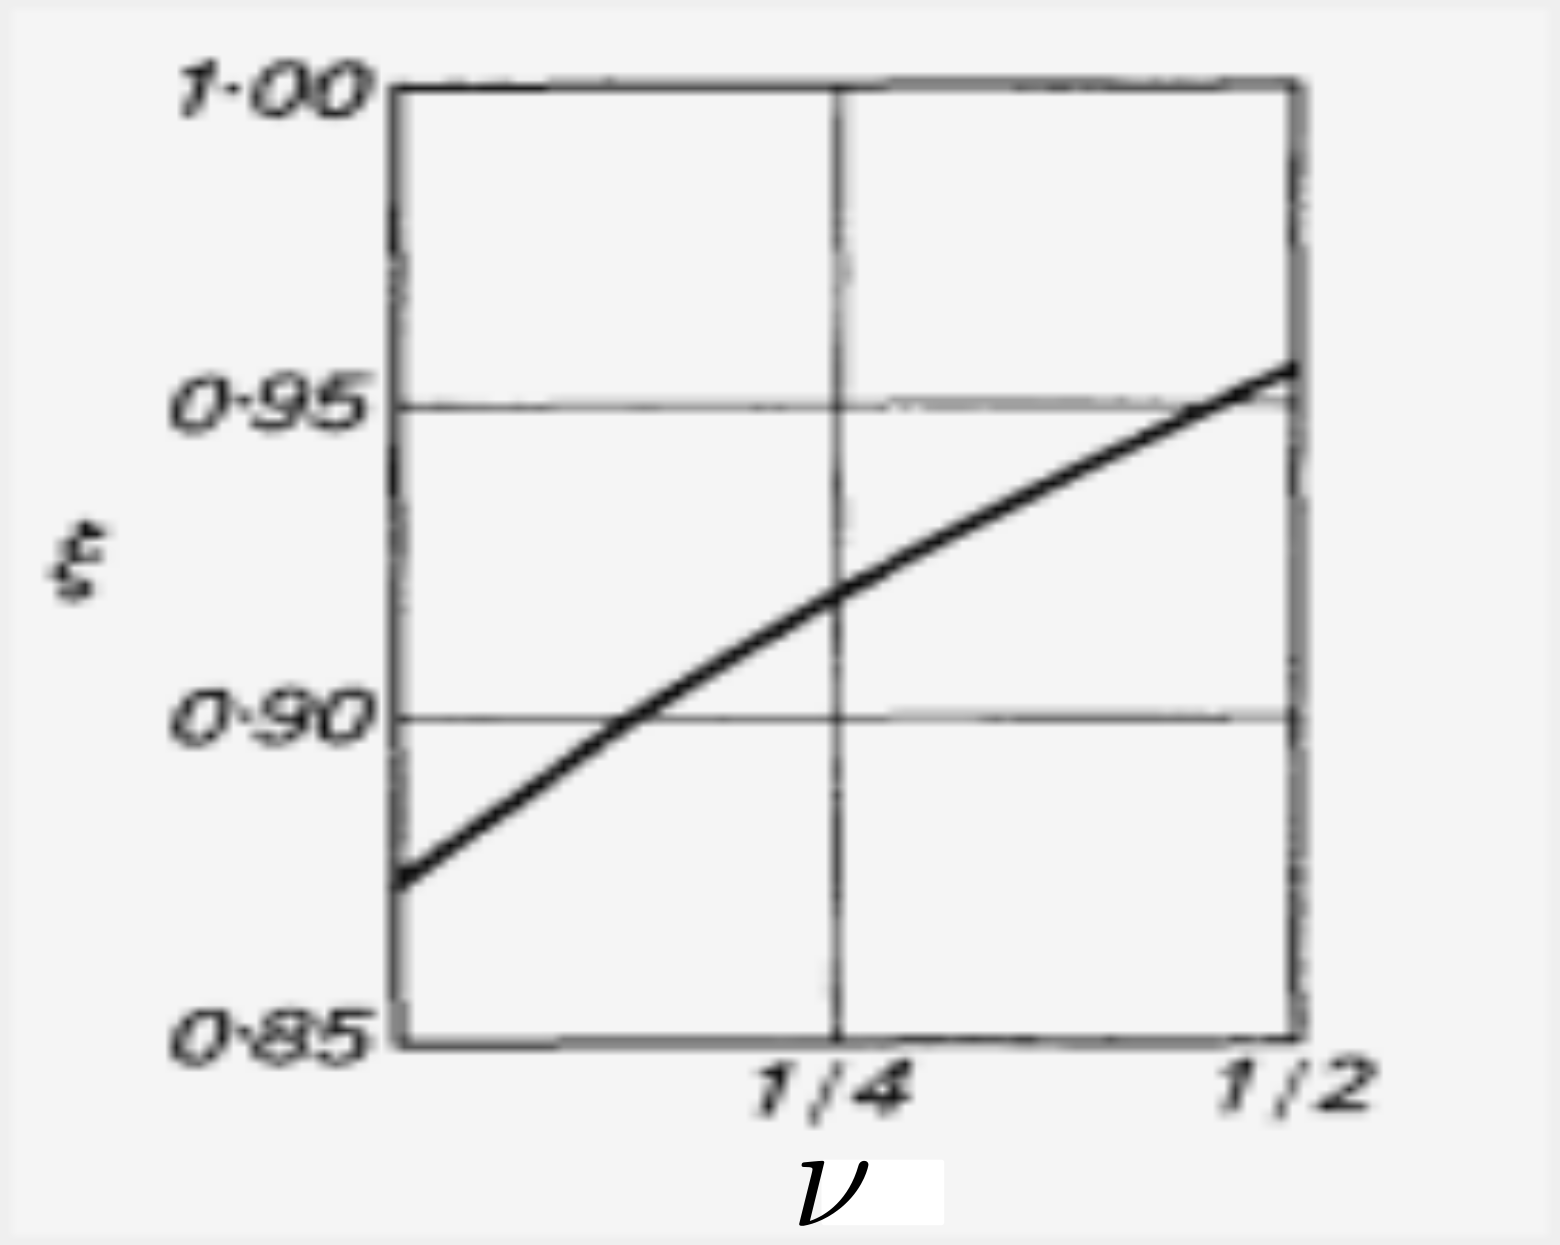
\includegraphics[width=0.5\textwidth]{fig/nu_xi.png}
	\caption{$\xi$ の$\nu$ 依存性(\cite{landau}より引用)}
	\label{fig:fig-nu_xi-png}
\end{figure}
以上まとめて\eqref{eq:55}\eqref{eq:58}\eqref{eq:73}から結局、格子変位$\bm{u}=(u_x,u_y,u_z)$ は以下のように計算できる。
\begin{equation}
\label{eq:74}
	u_x=u_0\left( -\sqrt{1-\xi^2} \exp (ikx+\kappa_t y-i\omega t)+\frac{2\sqrt{1-\xi^2} }{2-\xi^2}\exp (ikx + \kappa_l y -i\omega t) \right) 
.\end{equation}

\begin{equation}
\label{eq:75}
	u_y=iu_0\left( \exp (ikx+\kappa_t y-i\omega t)-\frac{2\sqrt{1-\xi^2} \sqrt{1-\xi^2(c_t^2 / c_l^2)} }{2-\xi^2}\exp (ikx+\kappa_ly-i\omega t) \right) 
.\end{equation}
\begin{equation}
\label{eq:76}
	u_z=0
.\end{equation}
ここで$u_0$ は対応する振幅であり、これらの一番目の項が横波に対応し、二番目の項が縦波である。
\section{スピン渦度結合によるスピン流生成}
\subsection{スピン流}
金属中には非常に高い密度の伝導電子がいて自由電子は物質中を高速で運動している。この伝導電子系に電場を与えると、電子の集団はある方向に
流れることになり、これが電流である。このとき通常の磁性を持たない金属ではスピンの向きはランダムに分布しているのでスピンの流れは
全体で打ち消されている。一方で例えばアップスピンの電子とダウンスピンの電子が同数でそれぞれ逆向きに運動している場合を考えると、これは電荷の流れとしては打ち消しあっていて正味の電流は$0$ である。一方でスピンの流れは打ち消されずに残る。このようなスピン角運動量の流れをスピン流といい、
特に上記の例のように電流が$0$ でスピン流だけが流れている状態を純スピン流状態という。
スピンの$z$ 成分が良い量子数の場合スピン流の$z$成分は$z$ 方向に平行なスピンを持つ電流$\bm{j}_{\uparrow}$ と$z$ 方向に反平行なスピンをもつ電流$\bm{j}_{\downarrow}$の差で表現され
\begin{equation}
\label{eq:77}
	\bm{J}_s=-\frac{\hbar}{2e}(\bm{j}_{\uparrow}-\bm{j}_{\downarrow})
.\end{equation}
ここで$e>0$ は電気素量である。一方で電流は
\begin{equation}
\label{eq:78}
	\bm{J}_c=\bm{j}_{\uparrow}+\bm{j}_{\downarrow}
.\end{equation}
と書ける。
スピン流と電流の決定的な違いは電流が一般に保存流であることに対してスピン流は保存流でないということである。
電荷保存則によって電流は保存流であるが、スピンに対しては保存則はなく、例えばSOIによってある確率で自然にスピンの向きが無秩序に変化してしまう。その結果電子スピン流はある程度の距離を流れると消えてしまう。この距離をスピン拡散長とよび、通常の金属では長くてもマイクロメートルスケールである。
\subsection{スピン蓄積}
空間的に非一様なスピン密度があると拡散スピン流が流れる。また電場$\bm{E}$ をかけるとドリフトスピン流が流れる。まずスピン自由度を考慮しないで考えると電流密度$\bm{j}$はドリフト流$\bm{j}_\text{drift} $と拡散流$\bm{j}_\text{diffusion} $ の和、$\bm{j}=\bm{j}_\text{drift} +\bm{j}_\text{diffusion} $で以下のように書かれる
\begin{equation}
\label{eq:79}
	\bm{j}=\sigma \bm{E}+eD\nabla n
.\end{equation}
ここで$\sigma$ は電気伝導度であり、$D$ は拡散係数、$n$ は粒子数密度である。
$\bm{j}_\text{drift} =\sigma \bm{E}$で$\bm{j}_\text{diffusion} =eD\nabla $であり、
フェルミエネルギー$E_F$ での状態密度を$N(E_F)$と書くと 化学ポテンシャル$\mu^{c}$ と粒子数密度には
\begin{equation}
\label{eq:80}
	N(E_F)\nabla \mu^{c}=\nabla n
\end{equation}
の関係が成り立ち、電気化学ポテンシャル$\phi$ を電位$\phi$ と化学ポテンシャル$\mu^{c}$ を用いて$\mu:=\mu^{c}-e\phi$ のように定義するとその勾配は
\begin{equation}
\label{eq:81}
	\nabla \mu = e\bm{E}+\frac{\nabla n}{N(E_F)}
.\end{equation}
したがって$\nabla \mu = 0$のとき電流密度
\begin{equation}
\label{eq:82}
	\bm{j}=(\sigma-e^2N(E_F)D)\bm{E}
\end{equation}
が$0$ であるとすれば以下のEinsteinの関係式が得られる。
\begin{equation}
\label{eq:83}
	\sigma=e^2N(E_F)D
.\end{equation}
\eqref{eq:81}と\eqref{eq:83}から次のようになる。
\begin{equation}
\label{eq:84}
	\bm{j}=\frac{\sigma}{e}\nabla \mu
.\end{equation}
この関係式は電気化学ポテンシャルの勾配$\nabla \mu$ が電流の駆動力となっていることを示している。
ここでスピンの自由度を再び考える。スピン流の駆動力となるのはスピン依存した電気化学ポテンシャル$\mu_{\sigma}$の勾配のアップスピン($\sigma=\uparrow$)とダウンスピン($\sigma=\downarrow$)の差である。
スピン依存した電流密度$\bm{j}_{\sigma}$ は以下のように表される。
\begin{equation}
\label{eq:85}
	\bm{j}_{\sigma}=\frac{\sigma_{\sigma}}{e}\nabla \mu_{\sigma}
.\end{equation}
ここで$\mu_\sigma= \mu_{\sigma}^{c}-e\phi$ はスピン依存電気化学ポテンシャルである。
電流とスピン流は\eqref{eq:77}、\eqref{eq:78}より
\begin{equation}
\label{eq:86}
	\bm{J}_c=\frac{1}{e}\nabla (\sigma_{\uparrow}\mu_{\uparrow}+\sigma_{\downarrow}\mu_{\downarrow})
.\end{equation}
\begin{equation}
\label{eq:87}
	\bm{J}_s=-\frac{\hbar}{2e^2}\nabla (\sigma_{\uparrow}\mu_{\uparrow}-\sigma_{\downarrow}\mu_{\downarrow})
.\end{equation}
特に非磁性体内では$\sigma_{\uparrow}=\sigma_{\downarrow}=\sigma$ なのでスピン流$\bm{J}_{s}$ は
\begin{equation}
\label{eq:88}
	\bm{J}_s=-\frac{\hbar\sigma}{2e^2}\nabla (\mu_{\uparrow}-\mu_{\downarrow})=-\frac{\hbar\sigma}{2e^2}\nabla \delta\mu
.\end{equation}
ここに$\delta\mu:=\mu_{\uparrow}-\mu_{\downarrow}$ はスピン蓄積とよばれ、スピン流を流すためのポテンシャルとなっている。
\subsection{スピン渦度結合}
スピン渦度結合(SVC)とはスピン角運動量と格子回転による渦度の結合でありハミルトニアンは
\begin{equation}
\label{eq:s1}
	H_{SVC}=-\bm{S}\cdot \bm{\Omega}=-\frac{\hbar}{2}\bm{\sigma}\cdot \bm{\Omega}
\end{equation}
で与えられる。
SVCの起源は強磁性体におけるEinstein-de Haas効果およびBarnett効果にあり、それぞれ強磁性体を磁化させるとそれに応じて回転する効果およびその逆効果である強磁性体を回転させると磁化する効果である。
Barnett効果では強磁性体に見かけの有効磁場であるBarnett磁場$\bm{h}_\text{B} $が生じると考えられ、その大きさは剛体回転の角速度$\bm{\Omega}$を後述する磁気回転比$\gamma$ で割った値
\begin{equation}
\label{eq:s2}
	\bm{h}_\text{B} =\frac{\bm{\Omega}}{\gamma}
\end{equation}
で与えられる。すなわち力学的回転$\bm{\Omega}$ はその回転軸方向の有効磁場$\bm{h}_\text{B} $ と等価である。

上記の磁気回転効果を強磁性体から非磁性金属へ、そして剛体回転から弾性体の格子回転を利用した局所的な渦度へ拡張した理論がSVCである。
この局所的な渦度中の電子の運動、すなわち
非一様な加速度系での電子の運動を考えるにあたって一般共変なDirac方程式を考える必要がある。
曲がった時空間でのスピン$1 /2$ の粒子を記述するそのような基礎方程式は
\begin{equation}
\label{eq:89}
	\left[ i \gamma^{\mu}(p_{\mu}+eA_{\mu}-i\hbar \Gamma_{\mu})+mc \right] \Psi =0
.\end{equation}
ここで$c$は光速で$\hbar$はプランク定数、$m$ は電子の質量である。$A_{\mu}$ はU(1)ゲージポテンシャルであり、$\Gamma_{\mu}$ はスピン接続とよばれる量であり、計量$g_{\mu\nu}(x)$ によって決められる。
座標依存したClifford代数として
$\gamma^{\mu}=\gamma^{\mu}(x)$において、
\begin{equation}
\label{eq:90}
\acomm{\gamma^{\mu}(x)}{\gamma^{\nu}(x)}=2g^{\mu\nu}(x),\quad(\mu,\nu=0,1,2,3)
\end{equation}
が成り立つ。
以下では格子変形がつくる速度場$\bm{v}=\dot{\bm{u}}$ のもとでの一電子について考える。
この速度場$\bm{v}$ がゲージポテンシャル$\Gamma_{\mu}$ の源になる。ここで$\abs{\bm{v}}\ll c$ であると仮定する。
格子変形速度場の局所静止系から慣性系への座標変換は$d\bm{r}'=d\bm{r}+\bm{v}(x)dt$となり、世界線素$ds$は
\begin{equation}
\label{eq:91}
	ds^2=g_{\mu\nu}dx^{\mu}dx^{\nu}=(-c^2+\bm{v}^2)dt^2+2\bm{v}\cdot d\bm{r} dt + d\bm{r}^2
.\end{equation}
このとき計量は
\begin{equation}
\label{eq:92}
	g_{00}=-1+\frac{v^2}{c^2},\quad g_{0i}=g_{i0}=\frac{v_i}{c},\quad g_{ij}=\delta_{ij}
.\end{equation}
\eqref{eq:89}、\eqref{eq:92}から局所静止系でのDiracハミルトニアンが導かれ次のようになる。\cite{physrevb.96.020401}
\begin{equation}
\label{eq:93}
	H=\beta m c^2+c \bm{\alpha}\cdot \bm{\pi }-eA_0+\frac{1}{2}e \bm{A}\cdot \bm{v}-\frac{1}{2}\acomm{\bm{v}}{\bm{\pi }}-\frac{1}{2}\bm{\Sigma}\cdot  \bm{\omega}
.\end{equation}
ここで$\beta,\bm{\alpha}$はDirac行列$\gamma^{\mu}$ と$\gamma^{0}(x)=i\beta$、$\gamma^{j}(x)=i\beta\alpha_{j}$ の関係があり以下のように表される。
\begin{equation}
\label{eq:94}
\beta = \begin{pmatrix}I &O\\O&-I  \end{pmatrix},\quad \bm{\alpha}=\begin{pmatrix} O&\bm{\sigma} \\ \bm{\sigma}&O\end{pmatrix} 
.\end{equation}
ここに$I$ は単位行列で$O$ は零行列、$\bm{\sigma}$ はパウリ行列である。
\\また$\bm{\Sigma}$はスピン演算子であり、
\begin{equation}
\label{eq:95}
\Sigma_{ij}=\frac{1}{2}\varepsilon_{ijk}\begin{pmatrix} \sigma_k & O\\O&\sigma_k\\ \end{pmatrix} 
.\end{equation}
さらに$\bm{\pi }$ は運動量$\bm{p}$ とU(1)ゲージ場$\bm{A}$を用いて$\bm{\pi }=\bm{p}+e\bm{A}$と表される。
また$\bm{\omega}$ は
\begin{equation}
\label{eq:96}
	\bm{\omega}=\nabla \times \bm{v}
\end{equation}
で表される渦度と呼ばれる量である。
\eqref{eq:93}の最終項$\bm{\Sigma}\cdot \bm{\omega} /2$がSVCハミルトニアン$H_\text{SVC} $である。
ここで$\bm{v}$ がある定数ベクトル$\bm{\Omega}$ を用いて
\begin{equation}
\label{eq:97}
	\bm{v}=\bm{\Omega}\times \bm{r}
\end{equation}
と書かれている場合を考える。
\eqref{eq:6}、\eqref{eq:8}で考えた格子変位$\bm{u}$ を速度場$\bm{v}$ で置き換えて考えると
渦度$\bm{\omega}$ と角速度$\bm{\Omega}$ の間には
\begin{equation}
\label{eq:98}
	\bm{\omega} = 2\bm{\Omega}
\end{equation}
の関係が成立する。
このようなとき\eqref{eq:93}の$-\acomm{\bm{v}}{\bm{\pi }} /2$ は回転と軌道角運動量とのカップリングを表す式$-\bm{\Omega}\cdot (\bm{r}\times \bm{\pi })$ になり、また最終項のSVCの項はスピン回転結合の形で$-\bm{\Sigma}\cdot \bm{\Omega}$ となり、回転座標系でのDiracハミルトニアンの表式
\begin{equation}
\label{eq:99}
	H=\beta mc^2+c \bm{\alpha}\cdot \bm{\pi }-(\bm{r}\times \bm{\pi })\cdot \bm{\Omega}-eA_0-\bm{\Sigma}\cdot \bm{\Omega}
\end{equation}
が得られる。
この回転系のDirac方程式から陽電子の自由度を消去した電子の低エネルギー有効理論を求めると$1 /m$ のオーダーで
\begin{equation}
\label{eq:100}
	H^{(1 /m)}_e=\frac{\bm{\pi}^2}{2m}-eA_0-(\bm{r}\times \bm{\pi })\cdot \bm{\Omega}-\frac{e\hbar }{2m}\bm{\sigma}\cdot \bm{B}-\frac{\hbar}{2}\bm{\sigma}\cdot  \bm{\Omega}
\end{equation}
となり、運動項やCoriolis項およびZeeman項に加えてやはり最終項にはスピン回転結合が残る。
このスピン回転結合の項をZeeman項に押し込むと
\begin{equation}
\label{eq:101}
H^{(1 /m)}_e=\frac{\bm{\pi}^2}{2m}-eA_0-(\bm{r}\times \bm{\pi })\cdot \bm{\Omega}-\frac{e\hbar }{2m}\bm{\sigma}\cdot (\bm{B}+\mu_0 \bm{h}_\text{B})
\end{equation}
が得られ、\eqref{eq:s2}で表されるBarnett磁場が現れる。ここで$\mu_0$は真空の透磁率である。

このSVCによるスピン流生成機構はStern-Gerlachの実験と同様な原理で説明される。
Stern-Gerlachの実験では磁場勾配にそってアップスピンとダウンスピンが分裂し、スピン流をつくる。本実験では表面弾性波の渦度が膜厚方向に減衰していくことを利用して渦度勾配、すなわちSVCによる有効磁場の勾配を作り出し、スピン流を生成した。
ただしStern-Gerlachの実験と異なるのは、SVCによる渦度勾配は時間的にも空間的にも周期的に変化する交流であるので、生成するスピン流も交流スピン流となる点である。
\subsection{スピン渦度結合によるスピン流生成}
\label{sec224}
スピン渦度結合(SVC)によるスピン流生成を記述するスピン拡散方程式を導く。

格子の力学的回転運動の角周波数である$\bm{\Omega}$ は\eqref{eq:96}、\eqref{eq:98}により
\begin{equation}
\label{eq:102}
	\bm{\Omega}=\frac{1}{2} \nabla \times \dot{\bm{u}}
\end{equation}
と表される。
ここで\eqref{eq:31}\eqref{eq:32}より格子回転が横波を持つ場合に\eqref{eq:102}は消えずに残ることがわかる。
上記の設定と同様に$x$ 方向に伝播して$y$ 方向に減衰する$xz$ 平面内を伝播する表面弾性波を考えると
$\bm{\Omega}=(0,0,\Omega)$のようになり、$\Omega$ は\eqref{eq:74}\eqref{eq:75}\eqref{eq:76}より次のように計算される。
\begin{equation}
\label{eq:103}
	\Omega(x,y,t)=\frac{\omega^2u_0}{2c_t}\exp \left[ -\kappa_t y+i(kx-\omega t) \right] 
.\end{equation}
ただしここで$u_0 \xi$ を改めて$u_0$ と置き直した。
このように$z$ 軸方向の力学的回転$\Omega$が与えられたとき、SVCハミルトニアン\eqref{eq:s1}により回転軸方向に平行にそろう。このとき電子のエネルギーバンドの底は$\hbar \Omega /2$ だけ変化する。アップ(ダウン)スピンの電子数密度$n_{\uparrow(\downarrow)}$
は次のように与えられる。
\begin{equation}
\label{eq:104}
	n_{\uparrow(\downarrow)}=\int_{\pm \hbar \Omega /2}^{\mu_{\uparrow(\downarrow)}} d\varepsilon N_0(\varepsilon)
.\end{equation}
ここで$ N_0$は電子の状態密度であり、$\mu_{\uparrow(\downarrow)}$ はアップ(ダウン)スピンの化学ポテンシャルである。
簡単のため状態密度を定数として考えるとこのときのスピン密度は次のように評価される。
\begin{equation}
\label{eq:105}
	n_{\uparrow}-n_{\downarrow}\simeq N_0(\delta\mu-\hbar \Omega)
.\end{equation}
ここに$\delta\mu=\mu_{\uparrow}-\mu_{\downarrow}$は\eqref{eq:88}で定義したスピン蓄積である。
スピンは緩和がおこり、スピン緩和時間$\tau_\text{sf} $および拡散定数$D$を用いてこのスピン緩和のプロセスは次のように表される
\begin{equation}
\label{eq:106}
	\frac{\partial }{\partial t} (n_{\uparrow}-n_{\downarrow})=\frac{1}{\tau_\text{sf} }N_0\delta\mu+D \nabla ^2(N_0\delta\mu)
.\end{equation}
\eqref{eq:105}\eqref{eq:106}よりSVCを含んだスピン拡散方程式
\begin{equation}
\label{eq:107}
\left( \frac{\partial }{\partial t} -D \nabla ^2+\frac{1}{\tau_\text{sf} } \right) \delta\mu=\hbar\frac{\partial  \Omega}{\partial t} 
\end{equation}
が得られる。\eqref{eq:107}の右辺がSVC由来のスピン蓄積$\delta\mu$ のsource項であり、力学的回転の時間微分すなわち渦度の時間微分に比例する。スピン流の生成にはもうひとつの機構が提唱されており、Takahashiらは液体\ce{Hg}の流体運動による定常的な渦度から生成されるスピン流を観測し、渦度自体に比例するスピン流生成機構を実験的に検証した\cite{TakahashiR2016Shg}。この方法でのスピン流生成は後にMatuoらによって理論的な説明がなされており結局SVC由来のスピン拡散方程式\eqref{eq:107}は次のように拡張される\cite{PhysRevB.102.174413,physrevb.96.020401}。
\begin{equation}
\label{eq:108}
\left( \frac{\partial }{\partial t} -D \nabla ^2+\frac{1}{\tau_\text{sf} } \right) \delta\mu=\hbar\frac{\partial \Omega}{\partial t} -\frac{\hbar}{\tau_\text{sf} }\zeta\Omega
.\end{equation}
ここで$\zeta$ は力学的回転とスピンとの変換効率を表す規格化因子である。
ここに$\Omega$ の表式\eqref{eq:103}を代入して方程式を解き、得られたスピン蓄積から\eqref{eq:88}を計算すると$z$ 方向に偏極した交流スピン流$J_s$が次のように求まる\cite{PhysRevLett.119.077202,PhysRevB.87.180402,PhysRevB.102.174413}。
\begin{equation}
\label{eq:109}
J_s=\left(\tau_\text{sf} \omega-i\zeta  \right) J_s'e^{i(kx-\omega t)}:=\left( J_s^{\tau_\text{sf}} -iJ_s^{\zeta} \right) e^{i(kx-\omega t)}
.\end{equation}
ここで$\kappa_t y\ll 1$という表面付近のスピン流を考えるとすれば、$J_s'$ は$y$ に比例した形で次のように与えられる。
\begin{equation}
\label{eq:110}
	J_s' \simeq -\frac{\hbar^2\sigma\omega^3u_0}{2e^2c_t^2}\left( 1+\frac{\kappa_t^2\lambda_s^2}{1-\xi^2} \right) ^{-1 /4} \frac{\sqrt{1-\xi^2} }{\xi}\frac{y}{\lambda_s}
.\end{equation}
ここに$\lambda_s=\sqrt{D \tau_\text{sf} } $ はスピン拡散長である。
\eqref{eq:109}から見て取れるように、生成されるスピン流は$J_s^{\tau_\text{sf} }$ と記した$\tau_\text{sf} $に比例するの項と、
$J_s^{\zeta}$ と記した$\zeta$ に比例する項がありそれぞれ\eqref{eq:108}の渦度の時間微分と渦度それ自身に比例する項である。
もしも前者の機構が支配的であるとすれば、これは$\tau_\text{sf} $に比例するためにスピン軌道相互作用(SOI)が弱く、散乱が起こりにくい材料がスピン流生成に有利であることを表している。
一方で後者の機構の$\zeta$ に比例するスピン流生成のSOIの寄与についてははっきりとわかってはいない。
さらに
\eqref{eq:109}\eqref{eq:110}からSVC由来のスピン流強度は角周波数$\omega$ の3乗ないしは4乗に比例するということがわかる。
すなわち高い周波数の波を励起するほど、より高いスピン流強度が得られることを示している。
\section{磁気共鳴}
SVCによって生成したスピン流が強磁性体に流れ込むと後述するスピントランスファートルクによりスピン波が励起される。本実験ではここに外部磁場をかけて磁気共鳴を起こすことでスピン流を検出した。
\subsection{LLG方程式}
原子の磁気モーメント$\bm{\mu}$は原子の角運動量$\bm{L}$に比例し平行もしくは反平行になる。電子の場合には反平行となり
\begin{equation}
\label{eq:111}
	\bm{\mu}=-\gamma \bm{L}
\end{equation}
と書かれる。ここで$\gamma$ は磁気回転比と呼ばれる量であり、
\begin{equation}
\label{eq:112}
	\gamma=\frac{g\mu_0e}{2m}
\end{equation}
で表される。ここに$g>0$ は$g$ 因子であり電子スピンの場合ほぼ$2$ である。$\mu_0$ は真空の透磁率、$e>0$ は電気素量、$m$ は電子の質量である。磁気モーメント$\bm{m}$ が外部磁場$\bm{H}$ の中にあるとき、トルク
\begin{equation}
\label{eq:113}
	\bm{T}=\bm{\mu}\times \bm{H}
\end{equation}
がかかり、\eqref{eq:111}から磁気モーメントは角運動量を随伴するのでトルク$\bm{T}$ が角運動量変化を生む。すなわち
\begin{equation}
\label{eq:114}
	\frac{d \bm{\mu}}{dt}=-\gamma \bm{\mu}\times \bm{H}
.\end{equation}
あるいは単位体積あたりの磁気モーメントである磁化$\bm{M}$ で書くと
\begin{equation}
\label{eq:115}
	\frac{d \bm{M}}{dt}=-\gamma \bm{M}\times \bm{H}
.\end{equation}
これは磁化の変化方向が磁化と外部磁場の両方に直交する方向であり、磁化$\bm{M}$が外部磁場$\bm{H}$を軸に歳差運動をすることを表している。
例えば外部磁場$\bm{B}$を$z$ 軸方向にかけてはじめ磁化$\bm{M}$ が外部磁場から角度$\theta$だけ傾いた状態で$xz$ 平面内にあるとする。
このときまず
\eqref{eq:115}は次のようになる。
\begin{equation}
\label{eq:116}
	\dot{M}_x=-\gamma H M_y
.\end{equation}
\begin{equation}
\label{eq:117}
	\dot{M}_y=\gamma H M_x
.\end{equation}
\begin{equation}
\label{eq:118}
	\dot{M}_z=0
.\end{equation}
これを解くと
\begin{equation}
\label{eq:119}
	M_x(t)=\abs{\bm{M}}\sin \theta \cos (\omega_0 t)
.\end{equation}
\begin{equation}
\label{eq:119-2}
	M_y(t)=\abs{\bm{M}}\sin \theta \sin  (\omega_0 t)
.\end{equation}
\begin{equation}
\label{eq:120}
	M_z(t)=\abs{\bm{M}}\cos \theta
.\end{equation}
このように$M_z$は定数であり$M_x,M_y$ は角周波数
\begin{equation}
\label{eq:121}
	\omega_0=\gamma H
\end{equation}
で歳差運動していることがわかる。
しかしながら実際には外部磁場をかけても磁化が傾き角$\theta$ を変えないまま歳差運動し続けるということは起こらず、スピン軌道相互作用などを介した格子系へのエネルギー散逸により回転は減衰し、最終的に磁化$\bm{M}$ は外部磁場$\bm{H}$ の方向に倒れてくる。
このような緩和項を現象論的に導入した方程式が Landau、Lifshits、 Gilbertによって提案され、次のように書かれる。
\begin{equation}
\label{eq:122}
	\frac{\partial \bm{M}}{\partial t} =-\gamma \bm{M}\times \bm{H}+\frac{\alpha}{M}\left[ \bm{M}\times \frac{\partial \bm{M}}{\partial t}  \right] 
.\end{equation}
ここに$\alpha$ はギルバードダンピング定数とよばれ、歳差運動の減衰時定数$\tau$ をもちいて$\alpha\simeq 1 /(\tau\omega_0)=1 /(\tau\gamma H)$\cite{alma9926360528104034}と書かれ、$\alpha$が大きいほど$\tau$ は短くなり急速に減衰することを示している。
この\eqref{eq:122}をLandau-Lifshits-Gilbert(LLG)方程式という。

さらにこの磁化をもった強磁性体にスピン流が流れ込んだ場合を考える。
伝導電子のスピン角運動量が強磁性体の磁化に受け渡され磁化が回転する。
このときの受け渡されるトルクをスピントランスファートルク(Spin Transfer Torque: STT)という。
角運動量保存に相当する式
\begin{equation}
\label{eq:123}
\frac{\partial }{\partial t} \bm{M}(\bm{r})=-(-\gamma)\mathrm{div}\,\bm{J}_s(\bm{r})=\gamma\,\mathrm{div}\, \bm{J}_s(\bm{r}) 
\end{equation}
を強磁性体内で磁化が一様であるとして全体に対して積分すると
\begin{equation}
\label{eq:124}
	\frac{\partial }{\partial t} \int dV \bm{M}=\gamma \int dV \mathrm{div}\, \bm{J}_s
.\end{equation}
強磁性体の磁化は一様なので\eqref{eq:124}の左辺は強磁性体の磁気モーメント$\bm{M}V$ の時間変化$\partial \bm{M}V /\partial t$となり、
右辺は面積分の形に書き換えて
\begin{equation}
\label{eq:125}
	\frac{1}{\gamma}\frac{\partial }{\partial t} (\bm{M}V)=\int dS \bm{J}_S:=\Delta \bm{J}_s
.\end{equation}
ここで\eqref{eq:125}右辺の面積分$\Delta \bm{J}_s$ は磁性体に吸収されたスピン流であり、大きさは$\abs{j_s}\hbar /2e$で局所的な向きとしてはスピン偏極方向$\bm{\sigma}$ と逆方向を向くベクトルである。スピントランスファートルクは磁化$\bm{M}$ に垂直な成分で磁化を傾ける向き、すなわちdamping-likeな向きのみであると仮定すると
\begin{equation}
\label{eq:126}
	\Delta \bm{J}_{s\perp}=\bm{m}\times (\bm{m}\times \Delta \bm{J}_s)
.\end{equation}
ここで$\bm{m}$ は磁化$\bm{M}$ の単位ベクトルである。
このスピントランスファートルクを含めて書き直したLLG方程式は
\begin{equation}
\label{eq:127}
\frac{\partial \bm{M}}{\partial t} =-\gamma\bm{M}\times \bm{H}+\frac{\alpha}{M}\left[ \bm{M}\times \frac{\partial \bm{M}}{\partial t}  \right] +\bm{\tau}_\text{STT} 
.\end{equation}
ただし
\begin{equation}
\label{eq:128}
	\bm{\tau}_{\text{STT} }=C \bm{M}\times (\bm{M}\times \bm{\sigma})
\end{equation}
\begin{equation}
\label{eq:129}
	C=-\frac{\gamma\hbar g(\theta) \abs{j_s}}{2dM_s^2e}
\end{equation}
であり、ここに$d$ は磁性体の膜厚、$M_s$ は飽和磁化である。$g(\theta)$ はスピン注入効率とよばれスピン分極ベクトル$\bm{\sigma}$と磁化$\bm{M}$とのなす角$\theta$ に依存する量で以下のように書ける\cite{ku}。
\begin{equation}
\label{eq:s4}
	g(\theta)=\left[ -4+\frac{(1+P)^3(3+\cos \theta)}{4P^{3 /2}} \right] ^{-1}
.\end{equation}
ここで$P$はアップスピンとダウンスピンの数密度 $n_{\uparrow}, n_{\downarrow}$ で
\begin{equation}
\label{eq:s5}
P=\frac{n_{\uparrow}-n_{\downarrow}}{n_{\uparrow}+n_{\downarrow}}
\end{equation}
のように定義されるスピン分極率である。
\subsection{強磁性共鳴}
強磁性体が磁場$\bm{H}$の中に置かれると磁化はLLG方程式に従い歳差運動しながら緩和していく。ここで$\bm{H}$ に直角に同じ周波数$\omega_0$ の高周波磁場$\bm{h}$ を加えると、磁化は減衰することなく歳差運動を継続する。この歳差運動が空間的に一様で位相差がない場合、この現象を強磁性共鳴(ferromagnetic resonance: FMR)と呼ぶ。FMRを具体的に記述するために$y$ 方向を深さ方向にもつ薄板形強磁性体に、$x$ 方向に静磁場$H$ を、$yz$ 面内に円偏光交流磁場$\bm{h}_\text{rf} =(0,h_y,h_z)$ を印加する場合を考える。
磁化のダイナミクスは\eqref{eq:122}のLLG方程式に従い
\begin{equation}
\label{eq:130}
	\frac{\partial \bm{M}}{\partial t} =-\gamma\bm{M}\times \bm{H}_\text{eff}-\gamma \bm{M}\times \bm{h}_\text{rf} +\frac{\alpha}{M_s}\left[ \bm{M}\times \frac{\partial \bm{M}}{\partial t}  \right] 
.\end{equation}

ここで$\bm{H}_\text{eff} $ は有効磁場であり、実際に磁化$\bm{M}$ に働く磁場は外部磁場の他にいくつかの磁場を含むが、ここでは異方性磁場などは本実験で用いた$\ce{NiFe}$の場合には小さいとして反磁場$H_\text{d} $ のみを取り出して
\begin{equation}
\label{eq:131}
	\bm{H}_\text{eff} =\bm{H}+\bm{H}_d=\begin{pmatrix} H\\0\\0 \end{pmatrix} -\begin{pmatrix} N_x\\N_y\\N_z \end{pmatrix} \frac{\bm{M}}{\mu_0}
.\end{equation}
ここで$N_x,N_y,N_z$ は$N_x+N_y+N_z=1$ をみたす反磁場係数であり、$y$ 方向を深さ方向にもつ薄膜では$N_x,N_z\ll N_y\simeq 1$となる。
円偏向交流磁場$\bm{h}_\text{rf} $ 及び磁化$\bm{M}$ が角振動数$\omega$ で振動すると仮定し、それぞれ
\begin{equation}
\label{eq:132}
	\bm{h}_\text{rf} =\begin{pmatrix} 0\\h_y\\h_z \end{pmatrix} = \begin{pmatrix} 0\\h_{y0}e^{i\omega t}\\-ih_{z 0}e^{i\omega t} \end{pmatrix} 
,\end{equation}
\begin{equation}
\label{eq:133}
	\bm{M} =\begin{pmatrix} m_x\\m_y\\m_z \end{pmatrix} = \begin{pmatrix} M_s\\m_{y0}e^{i\omega t}\\-im_{z 0}e^{i\omega t} \end{pmatrix} 
\end{equation}
とおく。まず共鳴周波数$\omega_\text{res} $ と静磁場$H$ との関係を導く。\eqref{eq:130}において交流磁場の寄与である第二項が緩和項である第三項を打ち消すと考えることができ、\eqref{eq:132}\eqref{eq:133}を代入して$y,z$ 成分を整理すると
\begin{equation}
\label{eq:134}
\begin{pmatrix}  -i \omega  /\gamma&-H-(N_z-N_x) M_s /\mu_0 \\ H+(N_y-N_x) M_s /\mu_0 & -i \omega /\gamma\end{pmatrix} \begin{pmatrix} m_y \\ m_z \end{pmatrix} =0
\end{equation}
を得る。$m_y,m_z$が非自明な解を持つことから以下が導かれる。
\begin{equation}
\label{eq:135}
	\omega_\text{res} =\gamma \sqrt{\left( H+(N_z-N_x) \frac{M_s}{\mu_0} \right)\left( H+(N_y-N_x) \frac{M_s}{\mu_0} \right)  } 
.\end{equation}
\eqref{eq:135}はKittelの式とよばれる。

FMRにおけるエネルギー吸収については\eqref{eq:130}\eqref{eq:131}に\eqref{eq:132}\eqref{eq:133}を代入し、$m_y,m_z$ について整理すると
\begin{equation}
\label{eq:136}
\begin{pmatrix} m_y\\m_z \end{pmatrix} =\frac{\gamma M_s}{(\gamma H-i\alpha\omega+\gamma M_s /\mu_0)(\gamma H-i\alpha\omega)-\omega^2}\begin{pmatrix} \gamma H-i\alpha\omega&-i\omega\\i\omega &\gamma H-i\alpha\omega+\gamma M_s /\mu_0\end{pmatrix} \begin{pmatrix} h_y\\h_z \end{pmatrix} 
.\end{equation}
ただし十分に薄い薄膜を仮定し$N_x=N_z=0,\quad N_y=1$とした。
これを以下のように書き直す。
\begin{equation}
\label{eq:137}
\begin{pmatrix} m_y\\m_z \end{pmatrix} :=\begin{pmatrix} \chi_{yy}&i\kappa\\-i\kappa&\chi_{zz} \end{pmatrix} \begin{pmatrix} h_y\\h_z \end{pmatrix} 
.\end{equation}
このように交流磁場に対する磁化の応答を表したとき、$\chi_{yy}=\chi_{yy}'-i\chi_{yy}''$, $\chi_{zz}=\chi_{zz}'-i\chi_{zz}''$, $\kappa=\kappa'-i\kappa''$ は複素磁化率と呼ばれ、$\alpha^2\ll 1$ の過程を用いて以下のように計算できる。
\begin{align}
	\chi_{yy}'&= \frac{\gamma^2M_s\left[ (\omega_\text{res} ^2-\omega^2)H+\alpha^2\omega^2(H+M_s /\mu_0) \right] }{\left[ \omega^2_\text{res} -\omega^2 \right] ^2+\left[ \alpha\gamma\omega(2H+M_s /\mu_0) \right]^2 } \\
	\chi_{yy}''&=\frac{\alpha\gamma M_s\omega\left[ (\gamma H)^2+\omega^2 \right] }{\left[ \omega^2_\text{res} -\omega^2 \right] ^2+\left[ \alpha\gamma\omega(2H+M_s /\mu_0) \right] ^2}\\
	\chi'_{zz}&= \frac{\gamma^2M_s\left[ (\omega^2_\text{res} -\omega^2)(H+M_s /\mu_0)+\alpha^2\omega^2H \right] }{\left[ \omega^2_\text{res} -\omega^2 \right] ^2+\left[ \alpha\gamma\omega(2H+M_s /\mu_0) \right]^2 } \\
	\chi''_{zz}&= \frac{\alpha\gamma M_s\omega\left[ (\gamma H+\gamma M_s /\mu_0)^2+\omega^2 \right] }{\left[ \omega^2_\text{res} -\omega^2 \right] ^2+\left[ \alpha\gamma\omega(2H+M_s /\mu_0) \right]^2 } \\
	\kappa'&= \frac{\gamma M_s \omega\left[ \omega^2_\text{res}-\omega^2  \right] }{\left[ \omega^2_\text{res} -\omega^2 \right] ^2+\left[ \alpha\gamma\omega(2H+M_s /\mu_0) \right] ^2} \\
	\kappa''&= \frac{\alpha\gamma M_s \omega^2\left[ 2\gamma H +\gamma M_s/\mu_0 \right] }{\left[ \omega^2_\text{res} -\omega^2 \right] ^2+\left[ \alpha\gamma\omega(2H+M_s /\mu_0) \right] ^2} 
.\end{align}
以上の結果からFMRによって磁化が交流磁場から吸収する単位時間、単位体積あたりのエネルギーは以下のように計算できる。
\begin{equation}
\label{eq:147}
	P_\text{FMR} =\frac{\omega}{2\pi }\int_{0}^{2\pi  /\omega}  \left[ \Im(\bm{H}_\text{eff}) \cdot \Im\left( \frac{\partial \bm{M}}{\partial t}  \right)   \right] dt=\frac{\omega}{2}\left[ \chi_{y}''h^2_{y0}+2\kappa'' h_{y0}h_{z 0}+\chi_{zz}''h^2_{z 0} \right] 
.\end{equation}
つまり磁化が吸収するエネルギーは複素磁化率の虚部によって決まり、周波数に関してLorentz関数形となる。

なお$\kappa''$ に比例する交差項は\eqref{eq:132}\eqref{eq:133}
で仮定したように交流磁場が円偏向磁場である場合に生じるエネルギー吸収であり、$h_y$ と$h_z$が同位相であるような直線偏向磁場である場合にはゼロになる。

\subsection{スピン波共鳴}
前節では磁化が一様ですべてのスピンが同位相で歳差運動する場合を考えたがこのような場合はむしろ特別であり、もしひとつのスピンが他と少しずれてしまったとすると隣のスピンは交換相互作用で平行になろうとしているためにこれもズレることになる。このズレは隣から隣へと伝わってゆき、このようにスピンすなわち磁化が位相をずらしながら歳差運動をするような現象をスピン波とよび、スピン波による磁気共鳴をスピン波共鳴(spin wave resonance: SWR)という。スピン波を記述するのに通常の波動と同じく波数ベクトル$\bm{k}$ を導入する。今$y$ 方向に深さをもつ薄膜で$x$ 方向に静磁場$H$ を印加し、同じく$x$ 方向に波数$k$ で伝搬するスピン波が励起されている場合を考える。このような静磁場とスピン波の波数ベクトルが平行なスピン波を後退体積波(backward volume wave: BVW)という。
BVWが励起されるとき、ある位置での磁化のダイナミクスは\eqref{eq:122}のLLG方程式に従い次のように表される。
\begin{equation}
\label{eq:148}
	\frac{\partial \bm{M}}{\partial t} =-\gamma \bm{M}\times \bm{H}_\text{eff} +\frac{\alpha}{M_s}\left[ \bm{M}\times \frac{\partial \bm{M}}{\partial t}  \right] 
.\end{equation}
ここで$\bm{H}_\text{eff} $ は\eqref{eq:130}\eqref{eq:131}のLLG方程式から磁化の間に働く交換磁場$\bm{h}_\text{ex} $ と双極子磁場$\bm{h}_\text{di} $ が付け加わって次のように書ける。
\begin{align*}
\label{eq:149}
	\bm{H}_\text{eff} &=\bm{H}+\bm{H}_\text{d} +\bm{h}_\text{rf} +\bm{h}_\text{ex} +\bm{h}_\text{di}\\
					  &=\begin{pmatrix} H\\0\\0 \end{pmatrix} +\begin{pmatrix} 0\\-M_s /\mu_0\\0 \end{pmatrix} +\begin{pmatrix} 0 \\ h_y \\h_z \end{pmatrix} +\frac{2A}{M_s^2}\nabla ^2\bm{M}+\nabla \int_{}^{} \frac{\nabla '\cdot \bm{M}(\bm{r}')}{\abs{\bm{r}-\bm{r}}'}d\bm{r}'
					  \stepcounter{equation}\tag{\theequation} 
.\end{align*}
ここで$A$ は交換定数であり、$N_x=N_z=0,\quad N_y=1$とした。
$x$ 方向に波数$k$ で伝搬するスピン波としての解は
\begin{equation}
\label{eq:150}
	\bm{M}=\begin{pmatrix} m_x\\m_y\\m_z \end{pmatrix} =\begin{pmatrix} M_s\\m_{y 0}(y)e^{-i(kx-\omega t)}\\ -im_{z 0 }(y)e^{-i(kx-\omega t)} \end{pmatrix} 
.\end{equation}
のようにおくことができるため、\eqref{eq:148}\eqref{eq:149}に代入すると次のようになる。
\begin{equation}
\label{eq:151}
	i\omega m_y=-\gamma \left( H+\frac{2A}{M_s^2}\left[ k^2-\frac{\partial ^2}{\partial y^2}  \right]  \right) m_z+\gamma(h_z+h^{z}_\text{di} )M_s-i\alpha\omega m_z
.\end{equation}
\begin{equation}
\label{eq:152}
	i\omega m_z=\gamma\left( H+\frac{2A}{M_s^2}\left[ k^2-\frac{\partial ^2}{\partial y^2}  \right]  \right) m_y-\gamma\left( h_y+h^{y}_\text{di} -\frac{M_s}{\mu_0} \right) M_s+i\alpha\omega m_y
.\end{equation}
これらの方程式を$m_y,m_z$ について解くことによって、BVWの周波数と静磁場の関係式を導くことができ、この関係式はBVWの周波数と波数の関係も記述することからBVWの分散関係と呼ばれる。薄板形強磁性体の膜圧$d$ 十分小さいとして、BVWの分散関係が以下のように求まる\cite{ku}。
\begin{equation}
\label{eq:153}
	\omega_\text{res} =\gamma \sqrt{\left( H+\frac{2A}{M_s}k^2 \right) \left( H+\frac{2A}{M_s}k^2+\frac{M_s}{\mu_0}\frac{1-e^{-kd}}{kd} \right) } 
.\end{equation}
なおBVWの波数$k$ が十分小さいとき、交換磁場$2Ak^2 /M_s$ が静磁場$H$ よりも十分小さいため、交換相互作用の寄与を無視できる。このようなBVWを特に静磁後退体積波(magnetostatic backward volume wave: MSVBVW)といい、MSBVWの分散関係は次のようになる。
\begin{equation}
\label{eq:154}
	\omega_\text{res} =\gamma \sqrt{H\left( H+\frac{M_s}{\mu_0}\frac{1-e^{-kd}}{kd} \right) } 
\end{equation}
$N_x=N_z=0,\quad N_y=1$ とした\eqref{eq:135}のKittlの式と比較すると実効的な反磁場が$(1-e^{-kd })/kd$ だけ小さくなっていることがわかる。
また複素磁化率およびMSBVWの励起によるエネルギー吸収についても前節のFMRの場合と同様に計算することができて
\begin{equation}
\label{eq:155}
	P_\text{MSBVW} =\frac{\omega}{2\pi }\int_{0}^{2\pi /\omega} \left[ \Im(\bm{H}_\text{eff} )\cdot \Im\left( \frac{\partial \bm{M}}{\partial t}  \right)  \right]  dt=\frac{\omega}{2}\left[ \chi_{yy}'' h^2_{y0}+2\kappa'' h_{y 0}h_{z 0}+\chi_{zz}'' h^2_{z 0} \right] 
.\end{equation}
ここで複素磁化率は前節のFMRの場合の結果において反磁場$M_s /\mu_0$の部分を$(1-e^{-kd}) /kd$だけ小さくなった実効的な反磁場に置き換えたものである。
\subsection{STTによるスピン波共鳴}
非磁性体(non-magnetic material: NM)と強磁性体(ferromagnetic material: FM)を使って、$y$ 方向を深さ方向にもつNM/FM/NMの3層膜を考える。 NM、FMはそれぞれスピン流生成層、検出層の役割を果たす。ここに$x$ 方向へ伝播するR-SAWが励起されると\ref{sec224}節で述べたように渦度勾配によってNM層に交流スピン流が生成され、FM層に注入される。そうすると\eqref{eq:128}\eqref{eq:129}で荒らされるスピントランスファートルク$\bm{\tau}_\text{SST} $が
磁化にかかるため、\eqref{eq:154}で表される分散関係を満たす静磁場を印加することによってスピン波が励起される(spin transfer torque spinwave resonance: STT-SWR)。
スピン流の空間分布がR-SAWの波数に一致するため、このスピン波の波数ベクトルはR-SAWの波数ベクトルに一致する。
\eqref{eq:128}\eqref{eq:129}で表されるSTTを以下のように変形する。
\begin{equation}
\label{eq:156}
	\bm{\tau}=-\gamma \bm{M}\times \bm{\bm{h}}_\text{STT} 
.\end{equation}
\begin{equation}
\label{eq:157}
\bm{h}_\text{STT} =\frac{\hbar g(\phi)\abs{j_s}}{2eMd}\bm{M}\times \bm{\sigma}=\frac{\hbar g(\phi)\abs{j_s}}{2eMd}\cos \phi e^{-i(kx-\omega t)}\bm{e}_y
.\end{equation}
ここで$\phi$ は$x$ 軸からの面内磁場印加角度であり、本実験の場合$\phi=0$である。$\bm{e}_y$ は$y$ 方向の単位ベクトルである。このようにSTTは深さ方向の有効磁場$\bm{h}_\text{STT} $ として磁化に作用する。従って\eqref{eq:155}より磁化が
\begin{equation}
\label{eq:158}
	P_\text{SWR}= \frac{\omega}{2}\chi_{yy}''\abs{\bm{h}_\text{STT} }^2 \propto \abs{j_s}^2g(\phi)^2\cos ^2\phi
\end{equation}
のエネルギーを吸収する。このとき吸収されたエネルギーを透過マイクロ波の減衰として電気的に測定することでスピン流を検出した。なお\eqref{eq:158}より減衰量がスピン流の大きさの2乗に比例するため、スピン流が時間的、空間的に交流でも検出が可能である。

\chapter{実験方法}
%\section{材料}
%\subsection{\ce{LiNbO3}}
%\subsection{\ce{Ni81Fe19}}
%\subsection{\ce{Pt}}
%\subsection{\ce{Mn}}
%\subsection{\ce{Ti}}
%\subsection{\ce{Au}}
\section{試料作製}
\subsection{素子設計}
本実験で用いた素子の概略図を図\ref{fig:IDT}に示す。
この素子は圧電基盤(\ce{LiNbO3})と基板上に成膜されたFM、NM層の膜、2つのすだれ状電極(Inter Digital Transducer: IDT)で構成されている。IDTは\ce{Ti}(3)/\ce{Au}(30)によって作製した(ここで括弧内の数字は\si{\nano \metre}単位の膜厚を表し、以下この表記を断りなく用いる)。
一対のIDT間の距離は\SI{460}{\micro \metre}であり、櫛幅および櫛間隔$d$は\SI{1}{\micro \metre}、\SI{2}{\micro \metre}、\SI{4}{\micro \metre}で櫛幅と櫛間隔が同じ長さになるように変化させた。このとき構造周期$\lambda$ はそれぞれ\SI{4}{\micro \metre}、\SI{8}{\micro \metre}、\SI{16}{\micro \metre}である。櫛の本数は11と17のものを作製した。

また一対のIDTの間にはFM層の膜として\ce{NiFe}を、NM層の膜としてスピンホール角の正負が異なる\ce{Mn}、\ce{Pt}を用いてそれぞれ
\ce{Pt}(6)/\ce{NiFe}(20)、\ce{Mn}(6)/\ce{NiFe}(20)、\ce{Pt}(40)/\ce{NiFe}(20)/\ce{Pt}(40)、\ce{Pt}(40)/\ce{NiFe}(20)/\ce{Mn}(40)の1辺\SI{400}{\micro \metre}の正方形の膜を作製した。


\begin{figure}[H]
	\centering
\begin{tikzpicture}
[
scale=1,
>=latex,
inner sep=0pt, outer sep=2pt,
temple/.style={color=black,opacity=1}
]
%\draw[step=0.25,gray,opacity=0.5] (0,0) grid (15,10);
\filldraw[fill=gray!50!blue!10,draw=black,opacity=1] (1,2) rectangle (14,9) ;
\draw[thick,fill=gray!30!blue!30] (1,2)--++(.25,-0.5)--(13.75,1.5)--(14,2)--(1,2)--cycle;
\filldraw[fill=lightgray,draw=black!50] (5.5,3.5) rectangle (9.5,7.5) ;
\draw[<->] (5.75,3.5)--(5.75,7.5)node[right, midway]{ \SI{400}{\micro \metre}}  ;
\draw[<->] (5.5,7.25)--(9.5,7.25) node [below, midway]{\SI{400}{\micro \metre}};
\node(L) at (7.5,2.5){\ce{LiNbO3}};


\filldraw[fill=gray!40!black!60,draw=black!50] (5.5,3.5)--++(.10,-.25)--++(3.8,0)--++(.10,.25)--++(-4,0)--cycle;
\filldraw[fill=yellow,draw=gray!80,opacity=1] (1.25,2.5)--(4.25,2.5)--(4.25,7.75)--++(-.25,0)--++(0,-5)--++(-.75,0)--++(0,5)--++(-.25,0)--++(0,-5)--++(-.75,0)--++(0,5)--++(-.25,0)--++(0,-5)--++(-.75,0)--++(0,-.25)--cycle;
\filldraw[fill=orange!50!yellow!40!lightgray,draw=gray!80] (1.25,2.5)--++(3,0)--++(-.1,-.25)--++(-2.8,0)--++(-.1,.25)--cycle;


\filldraw[fill=yellow,draw=gray!80] (1.25,8.5)--++(3.5,0)--++(0,-5.5)--++(-.25,0)--++(0,5)--++(-.75,0)--++(0,-5)--++(-.25,0)--++(0,5)--++(-.75,0)--++(0,-5)--++(-.25,0)--++(0,5)--++(-1.25,0)--++(0,.5)--cycle;

\filldraw[fill=yellow,draw=gray!80, opacity=1] (13.75,2.5)--++(-3,0)--++(0,5.25)--++(.25,0)--++(0,-5)--++(.75,0)--++(0,5)--++(.25,0)--++(0,-5)--++(.75,0)--++(0,5)--++(.25,0)--++(0,-5)--++(.75,0)--++(0,-.25);

\filldraw[fill=yellow,draw=gray!80] (13.75,8.5)--++(-3.5,0)--++(0,-5.5)--++(.25,0)--++(0,5)--++(.75,0)--++(0,-5)--++(.25,0)--++(0,5)--++(.75,0)--++(0,-5)--++(.25,0)--++(0,5)--++(1.25,0)--++(0,.5)--cycle;

\filldraw[fill=orange!50!yellow!40!lightgray,draw=gray!80] (10.75,2.5)--++(3,0)--++(-.1,-.25)--++(-2.8,0)--++(-.1,.25)--cycle;
\node(I1) at (3,8.25){IDT1};
\node(I2) at (12,8.25){IDT2};
\node(L) at (7.5,4.25){FM,NM};
\draw[<->] (12.75,3)--(12.75,7.75)node[right, midway]{ \SI{330}{\micro \metre}}  ;
\draw[<->] (10.25,5)--++(1,0)node[above, midway]{$\lambda$}  ;
\draw[<->] (4.75,8)--++(5.5,0)node[above, midway]{\SI{460}{\micro \metre}}  ;




\end{tikzpicture}

	\caption{実験に用いた素子の概略図}
	\label{fig:IDT}
\end{figure}
IDTは図\ref{fig:IDT}のように互い違いに櫛が並んでいる。IDTが成膜されている\ce{LiNbO3}は圧電基盤であり、ひずみを与えると電機分極が生じ(圧電効果)、逆に電場を加えるとひずみが生じる(逆圧電効果)。
このことからIDTの一方を接地し、もう一方を交流電源に接続することで、逆圧電効果により、IDTの構造周期と同じ長さの波長のR-SAWを励起することができる。
また励起されたR-SAWはFM、NM膜を通過した後、反対側のIDTの圧電効果によって検知できる。このように1対のIDTによってR-SAWを励起、検知する素子を遅延線形表面弾性波という。
\subsection{素子作製}
測定に用いた素子はリフトオフ法を用いて作製した。リフトオフ法とは基板上に均一に塗布されたレジストから成膜部分を取り除いた上で金属を蒸着し、後からレジストを剥がすことで基板に任意形状の薄膜を成膜する方法である。この素子作製の工程は図\ref{fig:sosisakusei}に示したとおりである。
\subsubsection{洗浄}
基板に付着したごみを取り除くため、\ce{LiNbO3}圧電基板をジメチルアセトアミド($\mathrm{ZDMAC}$)、アセトン、2-プロパノール(IPA)の順に浸して10分ずつ超音波洗浄を行った。超音波洗浄後に光学顕微鏡で表面の観察を行い、ごみが付着している場合は綿棒で表面をこすって取り除いた。
\subsubsection{レジスト塗布}
洗浄後、窒素ガンで乾燥させた基板に描画用のレジストをスピンコーターを用いて均一に塗布した。電子線描画とレーザー描画では波長が異なるため使用するフォトレジストの種類が異なる。IDTの作製は電子線描画で行い、FM、NM層の膜はマスクレス露光装置PALETを用いて行った。
まずは洗浄済みの基板を窒素ガンで乾燥させたあと、電子線描画用(EB)レジストを数滴たらし、スピンコーターを使って回転速度\SI{4000}{rpm}、\SI{90}{s}で均一に塗布した。EB用レジストはポジレジストZEP520-AとシンナーZEP-Aを2:1で混合した溶液である。その後シンナー除去や膜固定のために\SI{180}{\degreeCelsius}、\SI{180}{s}
の条件でプリベイクを行った。さらに圧電基板は絶縁性であり、
電子線の照射による基板のチャージアップを防ぐために、導電性コロイド(エスペーサー)をレジスト上に数滴垂らし、まず\SI{500}{rpm}、\SI{10}{s}、続いて\SI{1200}{rpm}、\SI{30}{s}の2段階回転で塗布した。

またマスクレス露光装置用のレジストにはAZ P1350を用いて回転速度\SI{2000}{rpm}、\SI{90}{s}で塗布した。レジストの水分の蒸発と膜固定のために\SI{100}{\degreeCelsius}で\SI{90}{s}プリベイクを行った。
\subsubsection{描画}
レジストを塗布した基板に電子線を照射し、設計したパターンを描画する手法を電子線描画(EB)という。電子線で照射されたレジスト部分が後述の現像の手順で抜け落ちる。EB装置は電子サイズでの微細なパターンを描画することができるため、ナノサイズのパターン作製が必要なIDTはEB装置を用いた。描画条件を表\ref{tab:1}に示す。
\begin{table}[H]
	\centering
	\caption{EBの描画条件}
	\label{tab:1}
	\begin{tabular}{ccc} \hline \hline
		加速電圧&電流量&ドーズ時間\\ \hline
		\SI{20}{kV}&\SI{320}{\pico \ampere}&\SI{2.5}{\micro \second} \\ \hline \hline
	\end{tabular}
\end{table}
一方FM、NM層の膜はEBに比べて装置の扱いが容易なマスクレス露光装置を用いて描画した。描画の条件を表\ref{tab:2}に示す。
\begin{table}[H]
	\centering
	\caption{マスクレス露光装置の露光条件}
	\label{tab:2}
	\begin{tabular}{cc} \hline \hline
		LEDパワー&露光時間\\ \hline
		\SI{26.5}{\%}&\SI{0.5}{\second} \\ \hline \hline
	\end{tabular}
\end{table}
\subsubsection{現像}
EB描画後の基板をまず超純水に約\SI{10}{s}浸し、エスペーサーを取り除いた。次に現像液ZED-N50に\SI{210}{s}、最後にリンス(固定液)ZMD-Bに\SI{60}{s}浸して描画部分のレジストを取り除いた。設計通りのパターンが描画されていることを光学顕微鏡で確認した。

マスクレス露光装置で描画した基盤は現像液AZ developerに\SI{25}{s}、リンスとして純水に\SI{30}{s}浸して描画部分のレジストを取り除き、光学顕微鏡で確認した。
\subsubsection{蒸着}
成膜は真空蒸着で行った。蒸着とは金属ターゲットを蒸発させて基板上に成膜する方法である。ターゲットの蒸気圧を上げ、不純物を取り除くために成膜室は高真空に保たれている。

IDTの成膜の際には\ce{Ti},\ce{Au}ターゲットを電子線で加熱、蒸発させて基板上に\ce{Ti}(3)/\ce{Au}(30)を成膜した。

FM、NM層の成膜の際には基板上に\ce{Pt}(6)/\ce{NiFe}(20)、\ce{Mn}(6)/\ce{NiFe}(20)、\ce{Pt}(40)/\ce{NiFe}(20)/\ce{Pt}(40)、\ce{Pt}(40)/\ce{NiFe}(20)/\ce{Mn}(40)を蒸着した。
\subsubsection{リフトオフ}
成膜後の基板を有機溶媒に浸し、レジストを溶解することによって基板上には描画した形の薄膜のみが残ることになる。この手順をリフトオフと呼ぶ。レジストが剥がれるまでZDMACに浸して必要に応じて超音波洗浄を行い、その後アセトン、IPAに浸して洗浄した。

\begin{figure}[H]
	\centering

\begin{tikzpicture}
[
scale=1.0,
>=latex,
inner sep=0pt, outer sep=2pt,
temple/.style={color=black,opacity=1}
]
%\draw[help lines,step=0.25] (0,0) grid (16,9);
%\foreach \x in {4,8,12}
%{
%\draw[red] (\x,0)--(\x,9);
%}
%\foreach \x in {3,6}
%{
%\draw[blue] (0,\x)--(16,\x);
%}
\foreach \x / \y [count=\i] in {0/9,4/9,8/9,12/9,0/6,4/6,8/6,12/6,0/3,4/3,8/3}
{
	\coordinate(p\i)at(\x,\y);
	\node at ($(p\i)+(.25,-.25)$) {\i};
}
\foreach \i in {1,2,...,11}
{
	\draw[fill=gray!50!blue!10,draw=black] ($(p\i)+(.25,-2.75)$) rectangle ++(3.5,.5) ;
}
\foreach \i in {2,3}
{
	\draw[fill=blue,draw=black] ($(p\i)+(.25,-2.25)$) rectangle ++(3.5,.5) ;
}

\foreach \i in {7,8}
{
	\draw[fill=pink] ($(p\i)+(.25,-2.25)$) rectangle ++(3.5,.75) ;
	
}

\foreach \i in {9,10}
{
	\draw[fill=pink] ($(p\i)+(.25,-2.25)$) rectangle ++(1.25,.75) ;
	\draw[fill=pink] ($(p\i)+(2.5,-2.25)$) rectangle ++(1.25,.75) ;
	
}

\foreach \i in {10}
{
	\draw[fill=gray] ($(p\i)+(.25,-1.5)$) rectangle ++(1.25,.5) ;
	\draw[fill=gray] ($(p\i)+(2.5,-1.5)$) rectangle ++(1.25,.5) ;
}

\foreach \i in {4,5}
{
	\draw[fill=blue] ($(p\i)+(.25,-2.25)$) rectangle ++(.25,.5) ;
	\draw[fill=blue] ($(p\i)+(3.5,-2.25)$) rectangle ++(.25,.5) ;
	\draw[fill=blue] ($(p\i)+(.75,-2.25)$) rectangle ++(.25,.5) ;
	\draw[fill=blue] ($(p\i)+(3,-2.25)$) rectangle ++(.25,.5) ;
	\draw[fill=blue] ($(p\i)+(1.25,-2.25)$) rectangle ++(1.5,.5) ;
}

\foreach \i in {5}
{
	\draw[fill=yellow] ($(p\i)+(.25,-1.75)$) rectangle ++(.25,.25) ;
	\draw[fill=yellow] ($(p\i)+(3.5,-1.75)$) rectangle ++(.25,.25) ;
	\draw[fill=yellow] ($(p\i)+(.75,-1.75)$) rectangle ++(.25,.25) ;
	\draw[fill=yellow] ($(p\i)+(3,-1.75)$) rectangle ++(.25,.25) ;
	\draw[fill=yellow] ($(p\i)+(1.25,-1.75)$) rectangle ++(1.5,.25) ;
}

\foreach \i in {5,6,...,11}
{
	\draw[fill=yellow] ($(p\i)+(.5,-2.25)$) rectangle ++(.25,.25) ;
	\draw[fill=yellow] ($(p\i)+(1.,-2.25)$) rectangle ++(.25,.25) ;
	\draw[fill=yellow] ($(p\i)+(2.75,-2.25)$) rectangle ++(.25,.25) ;
	\draw[fill=yellow] ($(p\i)+(3.25,-2.25)$) rectangle ++(.25,.25) ;
}

\foreach \i in {10,11}
{
	\draw[fill=gray] ($(p\i)+(1.5,-2.25)$) rectangle ++(1,.5) ;
}

\foreach \i in {3}
{
	\draw[->] ($(p\i)+(.625,-1)$)--++(0,-.75);
	\draw[->] ($(p\i)+(.625,-1)+(.5,0)$)--++(0,-.75);
	\draw[->] ($(p\i)+(.625,-1)+(2.25,0)$)--++(0,-.75);
	\draw[->] ($(p\i)+(.625,-1)+(2.75,0)$)--++(0,-.75);
	\node at ($(p\i)+(2,-1.375)$){電子線};
}
\foreach \i in {8}
{
	\draw[->] ($(p\i)+(2,-1)$)--++(0,-.5);
	\draw[->] ($(p\i)+(2.25,-1)$)--++(0,-.5);
	\draw[->] ($(p\i)+(1.75,-1)$)--++(0,-.5);
	\node at ($(p\i)+(2,-1.375)+(1.2,.25)$){レーザー光};
}


\node at ($(p1)+(.5,-.5)$) [right] {洗浄};
\node at ($(p2)+(.5,-.5)$) [right] {レジスト塗布};
\node at ($(p3)+(.5,-.5)$) [right] {電子線描画};
\node at ($(p4)+(.5,-.5)$) [right] {現像};
\node at ($(p5)+(.5,-.5)$) [right] {Ti/Au蒸着};
\node at ($(p6)+(.5,-.5)$) [right] {リフトオフ};
\node at ($(p7)+(.5,-.5)$) [right] {レジスト塗布};
\node at ($(p8)+(.5,-.5)$) [right] {レーザー描画};
\node at ($(p9)+(.5,-.5)$) [right] {現像};
\node at ($(p10)+(.5,-.5)$)[right] {FM,NM蒸着};
\node at ($(p11)+(.5,-.5)$)[right] {リフトオフ};

\end{tikzpicture}
	\caption{素子作製の工程}
	\label{fig:sosisakusei}
\end{figure}
\section{測定方法}
\subsection{ベクトルネットワークアナライザ測定}
本実験では被測定回路の高周波特性をベクトルネットワークアナライザ(Vector Network Analyzer: VNA)を用いて調べた。VNAにはPort1とPort2の2つの端子があり、2または1つの端子間の反射信号及び透過信号を測定することができる。VNAが測定できるパラメータはSパラメータとよばれ、本実験ではPort1からPort2への透過信号である$S_{21}$ を測定した。
信号は位相差と振幅をもった複素数で表示されSパラメータの絶対値$\abs{S}$ をデシベルで表す表記は$\mathrm{LogMag}\,S$とよばれ以下のように表される。

\begin{equation}
\label{eq:z1}
	\abs{S}\,\si{\decibel}=10 \log _{10}\left( \frac{\abs{P_\text{out} }\,/\si{\milli \watt}}{\abs{P_\text{in} }\,/\si{\milli \watt}} \right) \quad(\text{電力による表示})
.\end{equation}
\begin{equation}
\label{eq:z2}
	\abs{S}\,\si{\decibel}=20 \log _{10}\left( \frac{\abs{V_\text{out} }\,/\si{\volt}}{\abs{V_\text{in} }\,/\si{\volt}} \right) \quad(\text{電圧による表示})
.\end{equation}
また入力パワーを表す単位として\SI{1}{\milli \watt}を基準としたデシベル表示である\si{dBm}があり、
\begin{equation}
\label{eq:z3}
	\abs{x}\,\si{dBm}=10\log _{10}\left( \frac{\abs{P}\,/\si{\milli \watt}}{1 \,/\si{\milli \watt}} \right) 
.\end{equation}
の関係が成り立つ。本実験での入力パワーはすべて$P_\text{in} =\SI{-5}{dBm}=\SI{1e-0.5}{\milli \watt}=\SI{0.32}{\milli \watt}$で行った。

また、本実験では被測定試料に磁場を掃引し、周波数を変えて$S_{21}$ パラメータの変化を測定した。
\eqref{eq:158}の吸収エネルギーを評価するためにまず次のようなトレース演算を行った。
\begin{equation}
\label{eq:z4}
	\Delta P_{21}(f,H):=\abs{\bm{P}_{21}(f,H)-\bm{P}_{21}(f,H_\text{ref} )}
.\end{equation}
ここで$\bm{P}_{21}(f,H)$ は周波数$f$、掃引磁場$H$ における$S_{21}$ パラメータから計算される複素数表示した電力であり、$H_\text{ref} $ は参照磁場であり本実験で用いた\ce{NiFe}の磁化が飽和するのに十分な大きさである$\mu_0 H=\SI{30}{\milli \tesla}$とした。
このようなトレース演算をすることにより磁場に依存しない信号を取り除くことができる。
さらにこれを次のように規格化した。
\begin{equation}
\label{eq:z5}
\Delta P^{\text{norm}}(f,H):=\frac{\Delta P_{21}(f,H)}{P_\text{SAW} ^{\text{peak}}(H_\text{ref} )}
.\end{equation}
ここで$P_\text{SAW} ^{\text{peak}}(H_\text{ref} )$ は参照磁場$H_\text{ref} $での$\abs{\bm{P}_{21}(f,H_\text{ref} )}$ のpeak強度である。

このようにして得られた$\Delta P^{\text{norm}}(f,H)$ は分子分母がともにR-SAWの振幅$u_0^2$ に比例するため、$u_0$ に依存しなくなる。従って$\Delta P^{\text{norm}}(f,H)$を比較すれば、試料の個体差などによる$u_0$ のばらつきの影響を受けずに定量比較を行うことが可能となる。
\subsection{ゲーティング処理}
VNA測定で我々が評価したいのはIDTで励起されたR-SAWが最初にもう一方のIDTに到達した際の減衰量である。しかし実際にはR-SAWよりも十分速く伝わる電磁波やR-SAWの反射波などがあり、これらのノイズを取り除く必要がある。
そのため本実験ではVNAで測定する周波数依存の信号を高速逆フーリエ変換(inverse fast Fourier transform: IFFT)によって時間依存の信号に変換し、窓関数(window function)をかけてから、高速フーリエ変換(fast Fourier transform: FFT)によってもとの周波数依存の信号に戻すことにより、特定の時間領域の信号、すなわち励起されたR-SAWを最初に検知した時間領域の信号のみを取り出した。このような処理をゲーティング処理と呼ぶ。
この際用いた窓関数としては
\begin{equation}
\label{eq:z6}
	w(x)=0.54-0.46 \cos 2\pi x\quad(0\le x\le 1)
\end{equation}
で表されるhamming窓を用いた。
このゲーティング処理によって、不要応答である電磁波や多重反射波を取り除くことができる。
\subsection{測定系}
本実験における概略図を図\ref{fig:sokuteikei}に示す。VNAとIDT対をプローブコンタクトによって接続し、IDT1によって励起されたR-SAWが磁性層を通過した後IDT2によって検出される。この際に透過信号である$S_{21}$ パラメータをR-SAWの伝播方向に静磁場$H$を印加しながら測定し、その$S_{21}$ パラメータの変化からSTT-SWR\eqref{eq:158}を検出した。測定条件を表\ref{tab:3}に示す。
\begin{table}[H]
	\centering
	\caption{VNA測定条件}
	\label{tab:3}
	\begin{tabular}{ccccc|ccc}\hline \hline
		開始周波数&終了周波数&周波数点数&入力電力強度&バンド幅&開始磁場&終了磁場&磁場点数\\ \hline 
		\SI{10}{\mega \hertz}&\SI{2}{\giga \hertz}&3201&\SI{-5}{dBm}&\SI{700}{\hertz}&\SI{30}{\milli \tesla}&\SI{-30}{\milli \tesla}&301\\\hline\hline
	\end{tabular}
\end{table}

\begin{figure}[H]
	\centering
\begin{tikzpicture}
[
scale=0.8,
>=latex,
inner sep=0pt, outer sep=2pt,
temple/.style={color=black,opacity=1}
]
%\draw[step=0.25,gray,opacity=0.5] (0,0) grid (15,10);
\filldraw[fill=gray!50!blue!10,draw=black,opacity=1] (1,2) rectangle (14,9) ;
\draw[thick,fill=gray!30!blue!30] (1,2)--++(.25,-0.5)--(13.75,1.5)--(14,2)--(1,2)--cycle;
\filldraw[fill=lightgray,draw=black!50] (5.5,3.5) rectangle (9.5,7.5) ;
\filldraw[fill=gray!40!black!60,draw=black!50] (5.5,3.5)--++(.10,-.25)--++(3.8,0)--++(.10,.25)--++(-4,0)--cycle;
\filldraw[fill=yellow,opacity=1] (1.25,2.5)--(4.25,2.5)--(4.25,7.75)--++(-.25,0)--++(0,-5)--++(-.75,0)--++(0,5)--++(-.25,0)--++(0,-5)--++(-.75,0)--++(0,5)--++(-.25,0)--++(0,-5)--++(-.75,0)--++(0,-.25)--cycle;
\filldraw[fill=orange!50!yellow!40!lightgray] (1.25,2.5)--++(3,0)--++(-.1,-.25)--++(-2.8,0)--++(-.1,.25)--cycle;


\filldraw[fill=yellow] (1.25,8.5)--++(3.5,0)--++(0,-5.5)--++(-.25,0)--++(0,5)--++(-.75,0)--++(0,-5)--++(-.25,0)--++(0,5)--++(-.75,0)--++(0,-5)--++(-.25,0)--++(0,5)--++(-1.25,0)--++(0,.5)--cycle;

\filldraw[fill=yellow, opacity=1] (13.75,2.5)--++(-3,0)--++(0,5.25)--++(.25,0)--++(0,-5)--++(.75,0)--++(0,5)--++(.25,0)--++(0,-5)--++(.75,0)--++(0,5)--++(.25,0)--++(0,-5)--++(.75,0)--++(0,-.25);

\filldraw[fill=yellow] (13.75,8.5)--++(-3.5,0)--++(0,-5.5)--++(.25,0)--++(0,5)--++(.75,0)--++(0,-5)--++(.25,0)--++(0,5)--++(.75,0)--++(0,-5)--++(.25,0)--++(0,5)--++(1.25,0)--++(0,.5)--cycle;

\filldraw[fill=orange!50!yellow!40!lightgray] (10.75,2.5)--++(3,0)--++(-.1,-.25)--++(-2.8,0)--++(-.1,.25)--cycle;


\node(I1) at (3,8.25){IDT1};
\node(I2) at (12,8.25){IDT2};

\draw[fill=gray,opacity=0.7] (5,9.5) rectangle (10,11.5) ;
\node(VNA) at (7.5,10.5){交流電源};
\draw[thick] (5,10.5)--++(-3.5,0)--++(0,-2.25);
\draw[thick] (10,10.5)--++(3.5,0)--++(0,-2.25);
\draw[thick] (1.5,2.625)--++(0,-1.375);
\draw[thick] (1,1.25)--++(1,0);
\draw[thick] (1.125,1.125)--++(0.75,0);
\draw[thick] (1.125,1)--++(.75,0);
\draw[thick] (13.5,2.625)--++(0,-1.375);
\draw[thick] (1+12,1.25)--++(1,0);
\draw[thick] (1.125+12,1.125)--++(0.75,0);
\draw[thick] (1.125+12,1)--++(.75,0);

\draw[thick,red,->] (7.5-2.4,6)--(10,6) node[above,midway]{$H$};

\draw[thick,blue,->] (7.5-2.4,5.5)sin++(.6,.5)cos++(.6,-.5)sin++(.6,-.5)cos++(.6,.5)sin++(.6,.5)cos++(.6,-.5)sin++(.6,-.5)cos++(.6,.5);
\node[blue](RSAW) at (7.5,4.5){R-SAW};
\end{tikzpicture}
	\caption{STT-SWRの測定系}
	\label{fig:sokuteikei}
\end{figure}

\chapter{実験結果}
\chapter{考察}
\chapter{まとめ}
\chapter{謝辞}


\bibliographystyle{jplain}
\bibliography{bib}
\nocite{st,Peskin,spin_oxford,alma9926360528004034,alma990023076750204034,alma990023937250204034,ku,neko}

\end{document}
